
\documentclass[12pt]{article}
\usepackage{geometry}
\usepackage{amsmath,bm}
\usepackage{sectsty}
\usepackage{graphicx}
\usepackage{tabularx}
\usepackage{hyperref}
\usepackage{amsfonts}
\usepackage{url}
\usepackage{textcomp}
\setlength{\parskip}{1em}
\setlength{\parindent}{0 pt}
\usepackage[font=small,labelfont=bf]{caption}
%\numberwithin{equation}

\begin{document}
    \title{\noindent\textbf{Model-independent measurement of production of two jets with two charged lepton pairs in ATLAS detector at} $\mathbf{\sqrt{s} = 13\ {TeV}}$}
    \author{Dong Qichen}
    \maketitle

    \begin{abstract}
        \noindent Model-independent measurement of the cross-section and geometrical asymmetry of 
        inclusive production of two jets with two charged lepton pairs via two Z bosons in a fiducial 
        phase space with detector effect removed. Hint of electro-weak production of the process 
        is observed with background only hypothesis rejected with p-value 0.04 and significance $1.5\sigma$. 
        The measurement is 
        performed using $36fb^{-1}$ of proton proton collision data collected in the ATLAS detector 
        at the Large Hadron Collider. The result shows great consistency 
        with the standard model expectation. The fiducial phase space is further separated to an 
        electro-weak enhanced signal region and three strong process dominated control regions for further
        study.
    \end{abstract}
    \newpage

    \section{Introduction}
        \par Vector boson scattering (VBS) process is important as a pure electroweak interaction to 
        probe the nature of electroweak symmetry breaking\cite{dawson1999introduction} (EWSB). At the 
        TeV scale, VBS process violates the longitudinal unitarity without the higgs contribution; 
        however, in the standard model\cite{ALTARELLI:2005zv} (SM), the appearance of higgs boson cancels 
        the violation rigorously. Since higher-order effects beyond the SM (BSM) are suppressed tremendously 
        at low energy scale, the measurement of VBS process cross-section in higher energy scale may give hints of BSM theories which 
        offer alternative EWSB mechanisms to break the elegant cancellation. Moreover, 
        the study of the VBS process provides an excellent chance to observe the potential CP-violating effects\cite{peccei1995cp} beyond the SM 
        that contribute to the large matter-antimatter asymmetry observed in the universe. The potential CP violation effect comes from BSM interference
        since no CP violation is predicted by the SM in the VBS process.

        \par In the Large hadron collider (LHC)\cite{Evans:2008zzb}, VBS events are produced by a pair of vector bosons 
        radiated from the initial partons, the vector bosons then scattered with each other and form another pair of vector bosons. 
        At detector-level, events with two jets from the hadronization of gluons and quarks associated with two pairs of leptons originated from the second vector bosons pair 
        can be a signature of VBS process. Despite the complexity of final states, background processes other than the VBS can 
        also produce the same final state particles, we denote these processes $jjVV$, one of the main background of VBS process is $jjVV$ 
        production with strong interaction vertices ($Strong\ jjVV$). The most VBS concentrated channel is $jjVV$ processes with only electroweak interactions ($EW\ jjVV$). 

        \par The VBS process has been intensely studied in the ATLAS and CMS collaboration since 2016\cite{ALESSANDRO201844}. 
        the first observation of VBS process with significance $5.5\sigma$ is in $EW\ jjWW$ channel measured by CMS collaboration in 2017
        using $36fb^{-1}$ pp collision data\cite{PhysRevLett.120.081801}. The ATLAS collaboration observed VBS process in $EW\ jjZZ$ channel with significance $5.5\sigma$ 
        in 2019 using $139fb^{-1}$ pp collision data\cite{ATLAS-CONF-2019-033}. The results of these studies are all in agreement with the SM predictions.
        
        \par The $EW\ jjVV$ process in which both vector bosons decay leptonically is extremely rare with cross-section around $1fb$ in current energy scale, 
        but it is a relatively clean channel with minimal hadronic background and no missing momentum. In this report, only events with final states containing 
        two pairs of charged leptons from Z bosons was considered as signal, denote as $jjZZ4l$, other procedures were considered as backgrounds.
        Figure \ref{fig:feynman} shows example Feynman diagrams of leading order $Strong\ jjZZ$ and $EW\ jjZZ$ processes\cite{ATLAS-CONF-2019-033}.  
        \begin{figure}[ht]
            \begin{centering}
            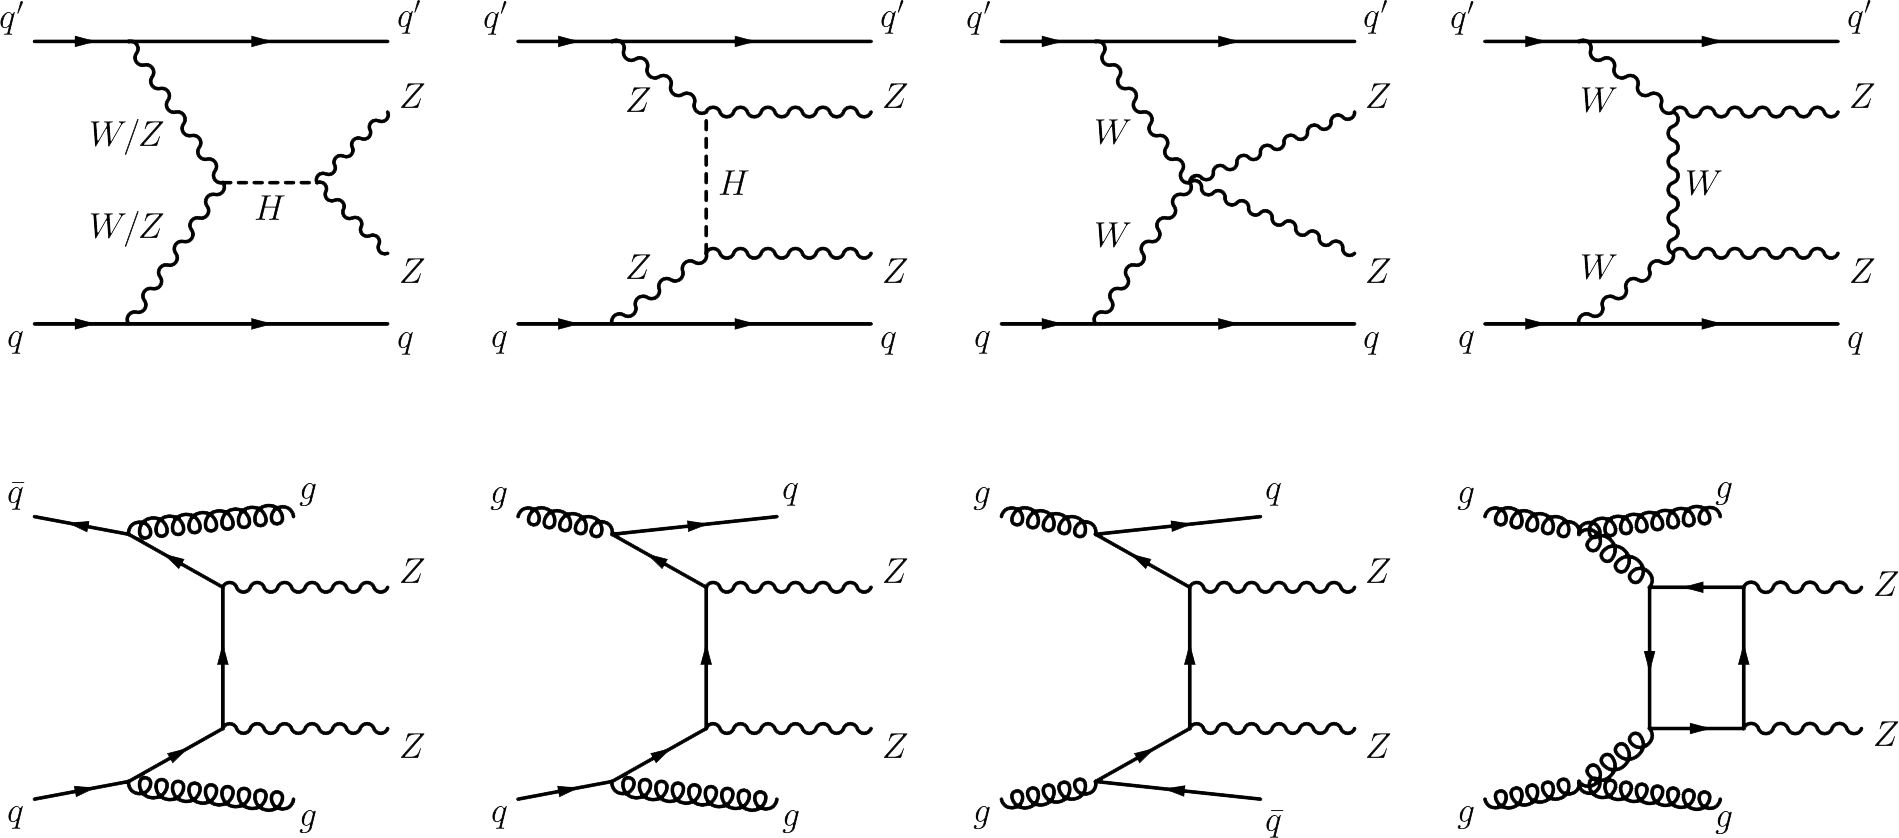
\includegraphics[scale=0.42]{ps/Feynman_diag.png}
            \caption{The first order feynman diagrams contributing to $jjZZ$ processes, the first line is $EW\ jjZZ$ and the second line is $Strong\ jjZZ$ processes.}
            \label{fig:feynman}
            \end{centering}
        \end{figure}
        \par Although the final state particles in leading order $EW\ jjZZ$ and $Strong\ jjZZ$ process is identical, the geometry configurations of them are quite 
        different, $EW\ jjZZ$ production process is expected to have a much larger jets separation since two heavy vector bosons emitted from each of the 
        initial state quarks. In contrast, the $Strong\ jjZZ$ production is expected to be more likely to radiate additional jets since the 
        colour charge carried by the quark or gluon is scattered backwards when emitting vector boson. It is likely for $Strong\ jjZZ$ process to have additional 
        hadronic interaction resulting additional jets between the two jets shown in leading order diagrams. Moreover, the vector bosons produced by 
        $EW\ jjZZ$ process are more centralised between the two associated jets and more balanced in momentum in transverse direction. These information are used 
        to define the signal region (SR) and control regions (CR) in this measurement.

        \par In this report, the $36 fb^{-1}$ pp collision data with centre-of-mass energy $\sqrt{s} = 13 TeV$ collected by the atlas detector in 2016 is used.
        The experimental effect induced by the detector inefficiency and limited resolution is removed by unfolding\cite{Cowan:2002in} using  
        simulated events. The inclusive $jjZZ4l$ process cross-section and a CP-sensitive geometrical asymmetry of jets configuration in a VBS enhanced 
        fiducial phase space is measured. The cross-section result is consistent with the SM prediction, and no CP violating effect is found in 
        the fiducial region. However, the results are free from detector effects, so that can be directly compared with theory predictions and 
        used to constrain various ``benchmark'' BSM theories.

    \section{ATLAS detector}
        \par The performance and geometry detail of ATLAS detector can be found in reference\cite{Collaboration_2008}. 
        ATLAS detector is a general-purpose layered-design particle detector constructed in 2008, which is cylindrically 
        symmetric to the beam axis with near complete coverage in solid angle. The first layer is the inner tracking 
        detector covering pseudorapidity range $|\eta| < 2.5$ submerged in 2T axial magnetic field produced 
        by superconducting electromagnet. It provides the ability to track charged particles and measure their momentum. 

        The second layer is the complex of the electromagnetic calorimeter and hadronic calorimeter both covering $|\eta| < 3.2$. An electron or photon
        interact with the liquid argon in the electromagnetic calorimeter and deposit energy through radiation, ionization and excitation, forming 
        a shower cone consisting of photons and electrons. The energy deposit and position information are then converted to electric signals.
        Hadrons undergo similar processes in the hadronic calorimeter, but the hadronic shower initiate by a high energy hadron through nuclear interactions has
        a much larger profile in both transverse and longitudinal direction.  
        In the region where $4.9> |\eta| > 3.2$, a forward electromagnetic and hadronic calorimeter is used. 
        
        The third layer is the large muon spectrometer covering $|\eta| < 2.7$. Since muons are much heavier than electrons, the radiation loss of them in the 
        electromagnetic calorimeter is much smaller, larger apparatus based on the ionization of muons have to be used to capture their tracks. 
        Around 25 $pp$ collides (2016) in the centre of the detector each time two beams of photon cross the detector, 
        resulting around 1 billion collisions per second, most of which are ``less interesting'' elastic collisions, 
        complicate hardware and software trigger system\cite{Nedden_2017} is used to select ``interesting'' inelastic collisions and cut down the
        rate to about 1000 per second for analysts to study. 
        A cut-away view of the ATLAS detector with main components labelled is shown in Figure \ref{fig:atlasdet}\cite{Collaboration_2008}.

        \begin{figure}[ht]
            \begin{centering}
            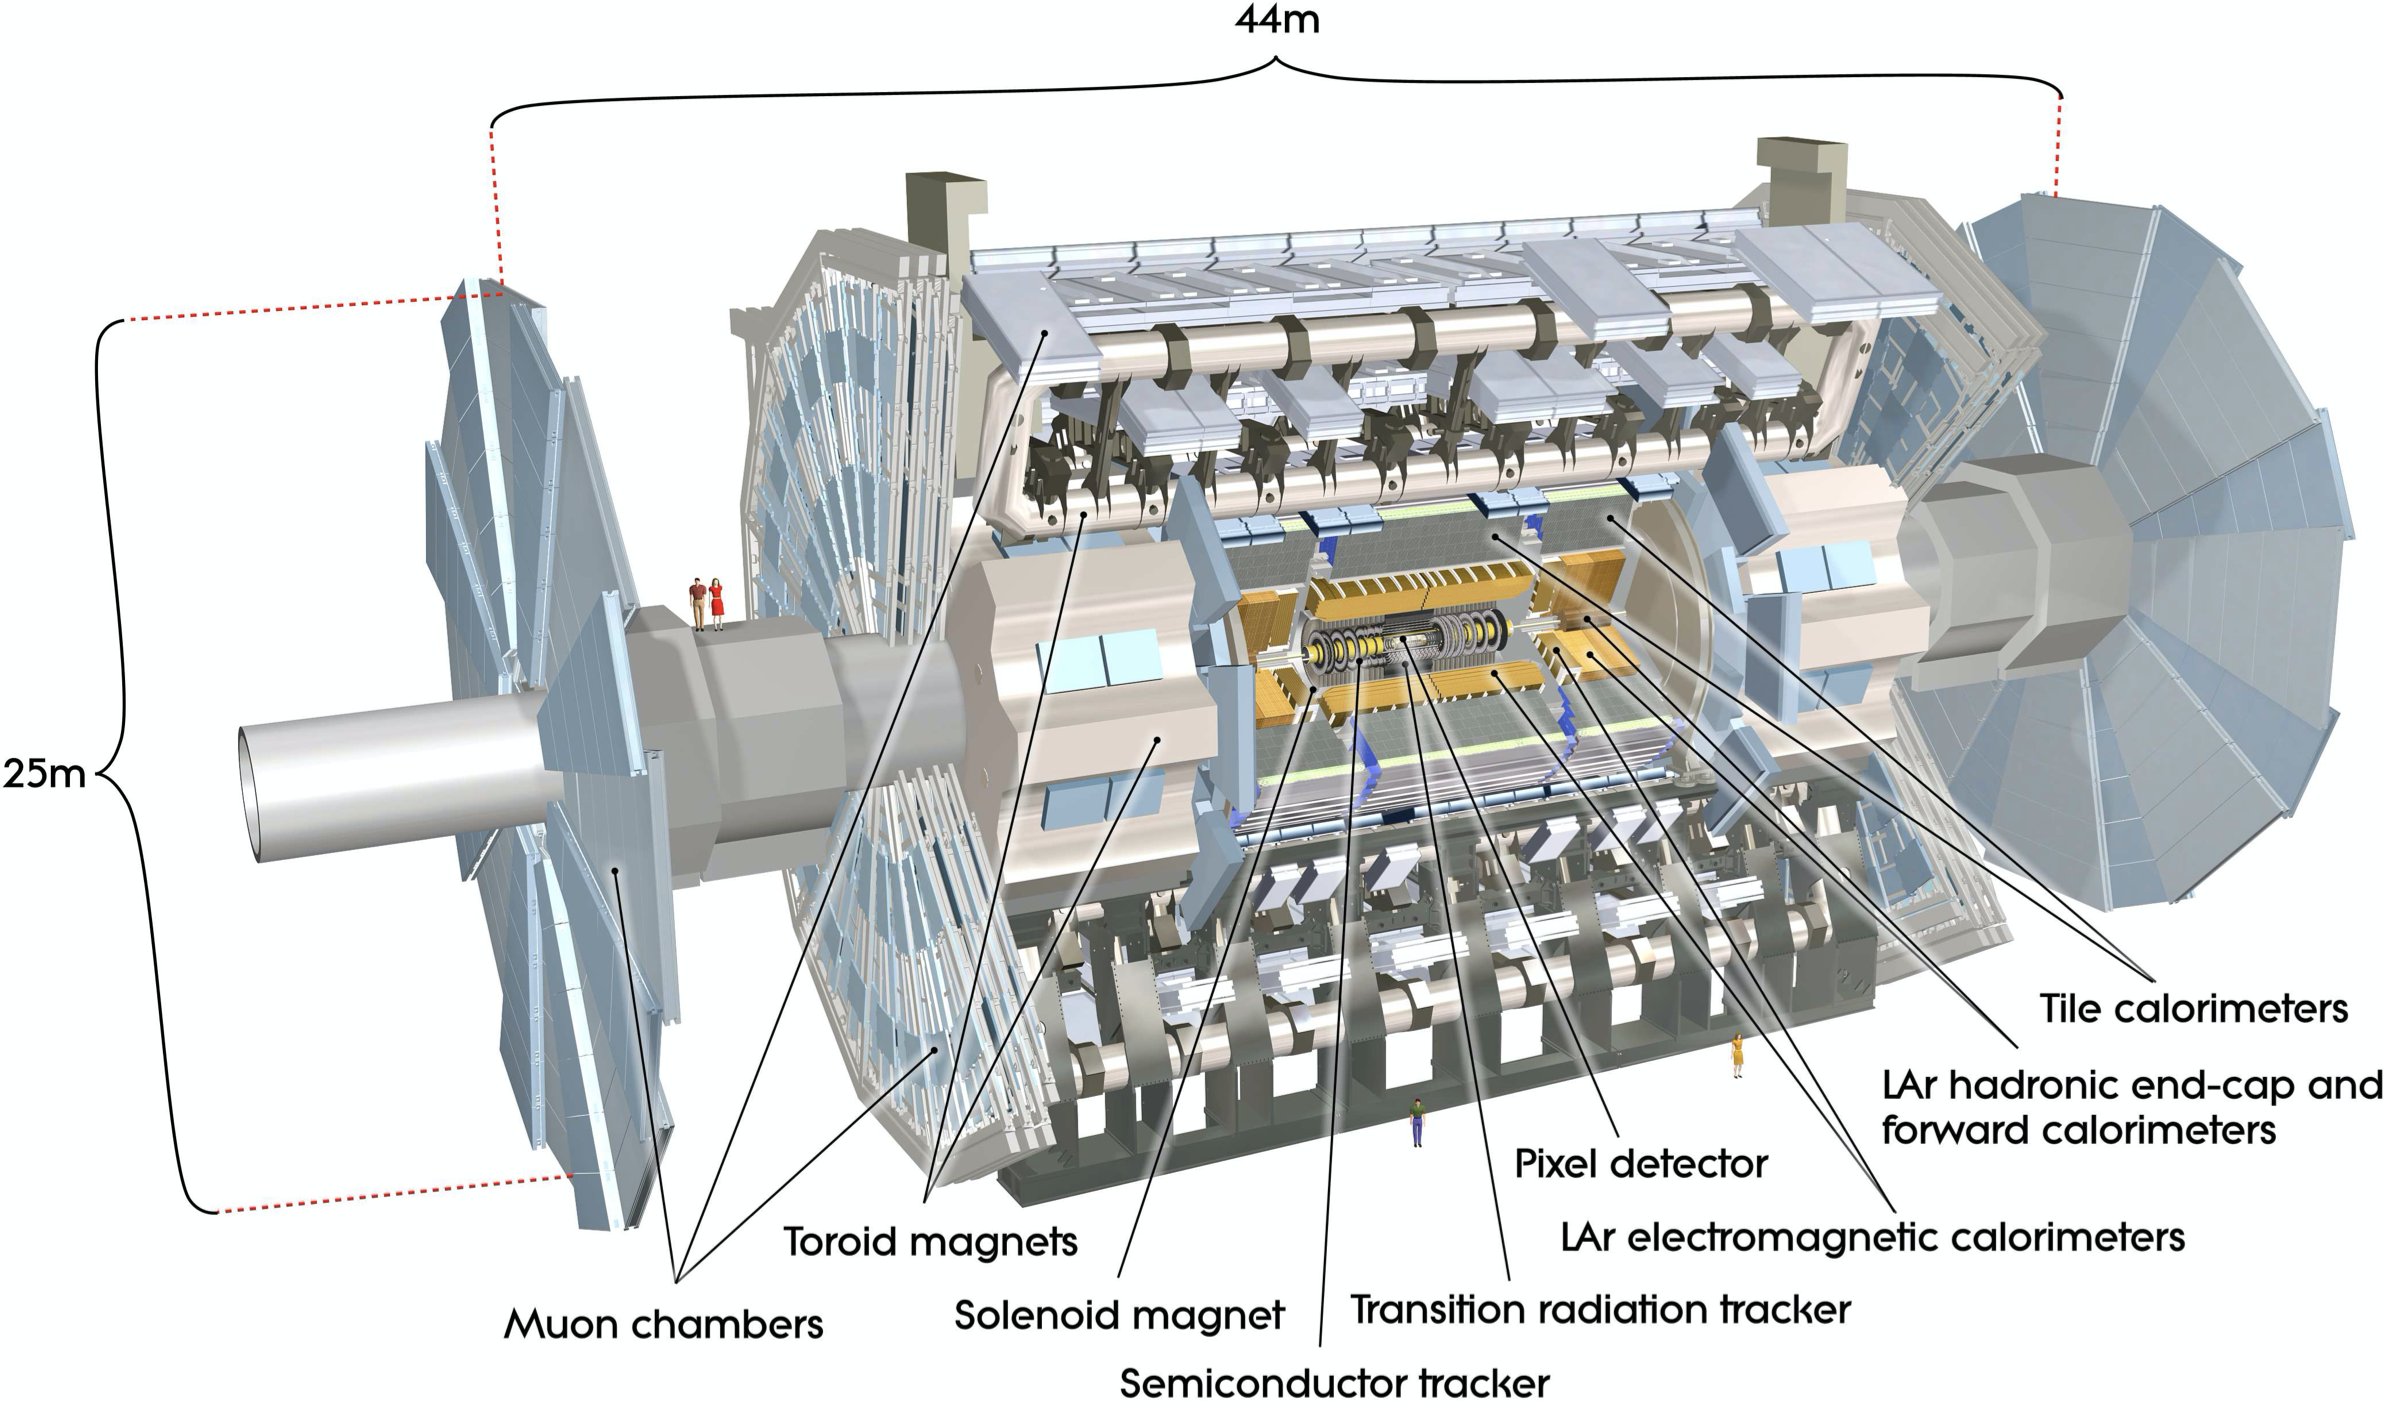
\includegraphics[scale=0.35]{ps/atlas_det.png}
            \caption{A cut-away view of the ATLAS detector, major components and the dimension of it is labelled.}
            \label{fig:atlasdet}
            \end{centering}

        \end{figure}
    \section{Data and Simulation}
        \par The measurement is performed using the pp collision data recorded during 2015 and 2016 run of LHC 
        with $\sqrt{s} = 13\ TeV$. During this period, an integrated luminosity of $36fb^{-1}$ is obtained. 
        Data taken in 2017 and 2018 run can be used in the future for further analysis.
        \par Simulations for various processes used in the measurement are generated by different Monte Carlo (MC) generators\cite{weinzierl2000introduction}\cite{Buckley2019MonteCE}, 
        three generations of simulation events corresponding to three years of LHC run with a different pile-up and integrated 
        luminosity are available, adding up to simulation data corresponding to a total luminosity of $139fb^{-1}$. 
        Only the simulation data corresponding to 2015 - 2016 run was used in this measurement to achieve the most accurate prediction to the data. 
        The $EW\ jjZZ$ process is modelled by Sherpa2.2.2\cite{0811.4622} with NNPDF3.0NNLO\cite{1405.0301} parton 
        distribution function (PDF) at leading order (LO). The vector boson fusion (VBF) higgs contribution is 
        modelled using POWHEGVBF\_H\cite{0911.5299} configuration with Pythia8\cite{1410.3012} showering and NNPDF3.0 
        PDF. The $Strong\ qq \rightarrow jjZZ$ process is generated by Sherpa2.2.2 with NNPDF30NNLO PDF, events with 
        less than two jets are generated at next to LO(NLO), others are generated at LO, while $t\bar{t}\rightarrow {H} \rightarrow ZZ$ 
        contribution is generated separately by POWHEG\cite{1007.3893} with Pythia8 showering and NNPDF2.3 PDF. The
         $Strong\ gg \rightarrow jjZZ$ process is modelled using Sherpa2.2.2 with NNPDF30NNLO PDF, again, the $gg\rightarrow {H}\rightarrow ZZ$ 
         is modelled separately with POWHEG and Pythia8.
        \par The production of $jjWZ$ events is produced by POWHEG with Pythia8. The EW tri-boson process with the same order of $\alpha=6$ is modelled by Sherpa2.2.2 with NNPDF30NNLO PDF. Single Z boson decay is modelled by Sherpa with NNPDF30NNLO PDF while $t\bar{t}Z$ decay is modelled separately with the same configuration. $t\bar{t}$ production is modelled by POWHEG with Pythia8 showering.
        \par All MC simulations include detailed detector simulation by Geant4\cite{AGOSTINELLI2003250}, for all $jjZZ$ processes, truth-level (without detector simulation) simulations are also provided. Both simulated events and the data were reconstructed using raw spacial information and momentum of leptons and jets using the CERN ROOT\cite{ANTCHEVA20092499} framework.

    \section{Candidates selection}
        \begin{table}[ht!]
            \centering
            \renewcommand\arraystretch{1.2}
            \begin{tabularx}{\textwidth}{X c} 
            \hline\hline
            Objects &  \begin{tabular}{p{2cm}  p{2cm}  p{2cm}  p{2cm}} SR & $\text{CR}_{C_{ZZ}}$ & $\text{CR}_{jIB}$ & $\text{CR}_{all}$ \end{tabular}\\ 
            \hline\hline
            Electrons & \begin{tabular}{c} ``Loose'' ID criterion\\ ``FixedCutPflowLoose'' criterion\\$p_T > 7 \text{\ GeV},\ |\eta| < 2.47$ \\ $|d_0/\sigma_{d_0}| < 5,\  |z_0 × \text{sin}\theta| < 0.5 \text{mm}$\end{tabular} \\
            \hline
            Muons & \begin{tabular}{c} ``Loose'' ID criterion\\ ``FixedCutPflowLoose'' criterion\\$p_T > 7 \text{\ GeV},\ |\eta| < 2.7$ \\ $|d_0/\sigma_{d_0}| < 3,\  |z_0 × \text{sin}\theta| < 0.5 \text{mm}$\end{tabular} \\
            \hline
            Jets &  $P_T > 30(40) \text{GeV}$ for $|\eta| < 2.4(2.4<|\eta| < 4.5)$ \\
            \hline
            OSFC lepton pairs & \begin{tabular}{c} two pairs of OSFC lepton with $M_Z$ closest to Z mass \\ $p_T > 20, 20, 10$ GeV for leading 3 leptons \\ $\Delta{R_{l^+l^-}} > 0.2$ \\$70\ \text{GeV}<M_{Z_1} < 110$ GeV \\ $21\ \text{GeV}<M_{Z_2} < 110$ GeV\end{tabular} \\
            \hline
            Dijets system & \begin{tabular}{c}leading two jets with $y_{j_1} \times y_{j_2} < 0$ and $|y_{j_1} - y_{j_2}| > 2$\\ dijet invariant mass $M_{jj} > 200$ GeV\end{tabular} \\
            \hline
             &  $P_{T\ balance} < 0.5$\\
            jjZZ system & \begin{tabular}{p{2cm}  p{2cm}  p{2cm}  p{2cm}} $C < 0.5$ & $C < 0.5$ & $C > 0.5$ & $C > 0.5$ \\ $nIBj = 0$ & $nIBj > 0$ & $nIBj = 0$ & $nIBj > 0$\end{tabular}\\
            \hline\hline
            \end{tabularx}
            \caption{Summary of selection applied for selecting events in SR and CR phase space.}
            \label{selectioncut}
        \end{table}
        \par Selecting the desired $ZZ4l$ events while subtracting other background effects is challenging while distinguishing 
        $EW\ jjZZ$ and $Strong\ jjZZ$ is even harder, the final states of both processes are identical, but we can still study 
        the differences in geometry information and possible associated process of these events. The selection used in this 
        report is mostly similar to the selection detailed in ref. \cite{ATLAS-CONF-2019-033}.
        \par The detector-level selection relies on the properties of all final state particles, namely charged leptons and jets.  
        \par A jet is defined as a collimated spray of stable particles arising from the fragmentation and hadronisation of a 
        parton after a collision\cite{Atkin_2015}. They are reconstructed by combining tracks and hadron calorimeter signals in a conical region.
        In $jjVV$ processes, jets originate from the initial partons and radiated hadrons. 
        Within $|\eta| < 2.4$, jets were required to have transverse momentum 
        ($p_{T}$) higher than 30 GeV, jets with higher pseudorapidity $2.4 < |\eta| < 4.5$ have $p_T > 40$ GeV. 

        \par Muons are identified by compatible tracks in the muon spectrometer and the inner tracking detector. 
        Outside the region of inner tracking detector, muons can also be identified by an MS track alone. 
        The identified muons described above were required to have $p_{T} > 7 $GeV. Muons were required to have 
        $|\eta| < 2.7$  and satisfy ``loose'' particle identification criterion. Electrons were identified using 
        the information of the EM calorimeter and corresponding tracks in the inner tracking detector. Electrons 
        were also required to satisfy ``loose'' identification working point, and have $p_{T} > 7 $GeV and $|\eta| < 2.47$.

        \par A ``FixedCutPflowLoose" lepton isolation creteria\cite{Aaboud_2019} was required by all identified charged 
        leptons to remove leptons overlap with jets. Furthermore, the tracks of leptons were required to have transverse 
        impact parameter $d_0$ and longitudinal impact parameter $z_0$ satisfying $d_0/\sigma_{d_0} < \text{5}$ and $z_0\text{sin}\theta < 0.5 \text{\ mm}$.
        \par The resonance of Z boson pair were reconstructed by two pairs of same flavour, opposite charge (denote SFOC) leptons, 
        the tracks of two SFOC lepton pairs were required have separation $\Delta R > 0.2$, where $\Delta R = \sqrt{{\Delta\eta}^2 + {\Delta\phi}^2}$, 
        moreover, the three leading leptons with higher $p_T$ were required to have $p_T > 20, 20, 10$ respectively. 
        If more then two candidate OSFC lepton pairs were available, the lepton pairs with invariant mass($m_{l^+l^-}$) 
        closest to Z boson mass were selected. The lepton pair with mass closest to Z boson mass were required to have 
        invariant mass $70GeV < m_{Z_1} < 110GeV$ and the other Z boson to have $21\ GeV < m_{Z_1} < 110GeV$.
        \par Events must have at least two jets, the leading and subleading jets with $y_{j_1} \times y_{j_2} < 0$, $|y_{j_1} - y_{j_2}| > 2$ 
        , dijet invariant mass $m_{jj} > 200 GeV$ and $P_{Tj_1} > P_{Tj_2}> 30 GeV$ were selected. 

        \par The $EW jjZZ$ events are predicted to be more balanced in transverse momentum $P_T$, which is parametrised by 
        $$P_{T\ balance} = |\frac{P_{T\ jjZZ}}{P_{T\ Z_1} +  P_{T\ Z_2} +  P_{T\ j_1} +  P_{T\ j_2}}|$$ 
        where the numerator is the total $P_T$ of the 4 leptons 2 jets system and the denominator is the 
        scalar sum of individual $P_T$. Events were required to have $P_{T\ balance} < 0.5$.

        \par With the fiducial phase space defined, signal region (SR) and control regions (CR) are further defined base on the centrality 
        and the appearance of additional jets in-between the leading and subleading jets (denote $nIBj$). 
        The centrality is defined as $$C_{ZZ} = \frac{y_{jj} - y_{ZZ}}{y_{j_1}-{y_{j_2}}}$$ which indicates how the Z boson pair system 
        is centralised in the dijet system. In the SR region, events are required to have $C < 0.5$ and $nIBj=0$, outside of which were 
        defined as conjugate CR. Table \ref{selectioncut} summarises the fiducial region, SR and CR definition used in the analysis.
        \par The truth-level phase spaces are the same as the detector-level, except the lepton ID and isolation 
        criterion, $d_0$ and $z_0$ which are not applicable in truth-level.
        \begin{figure}[ht]
            \begin{centering}
            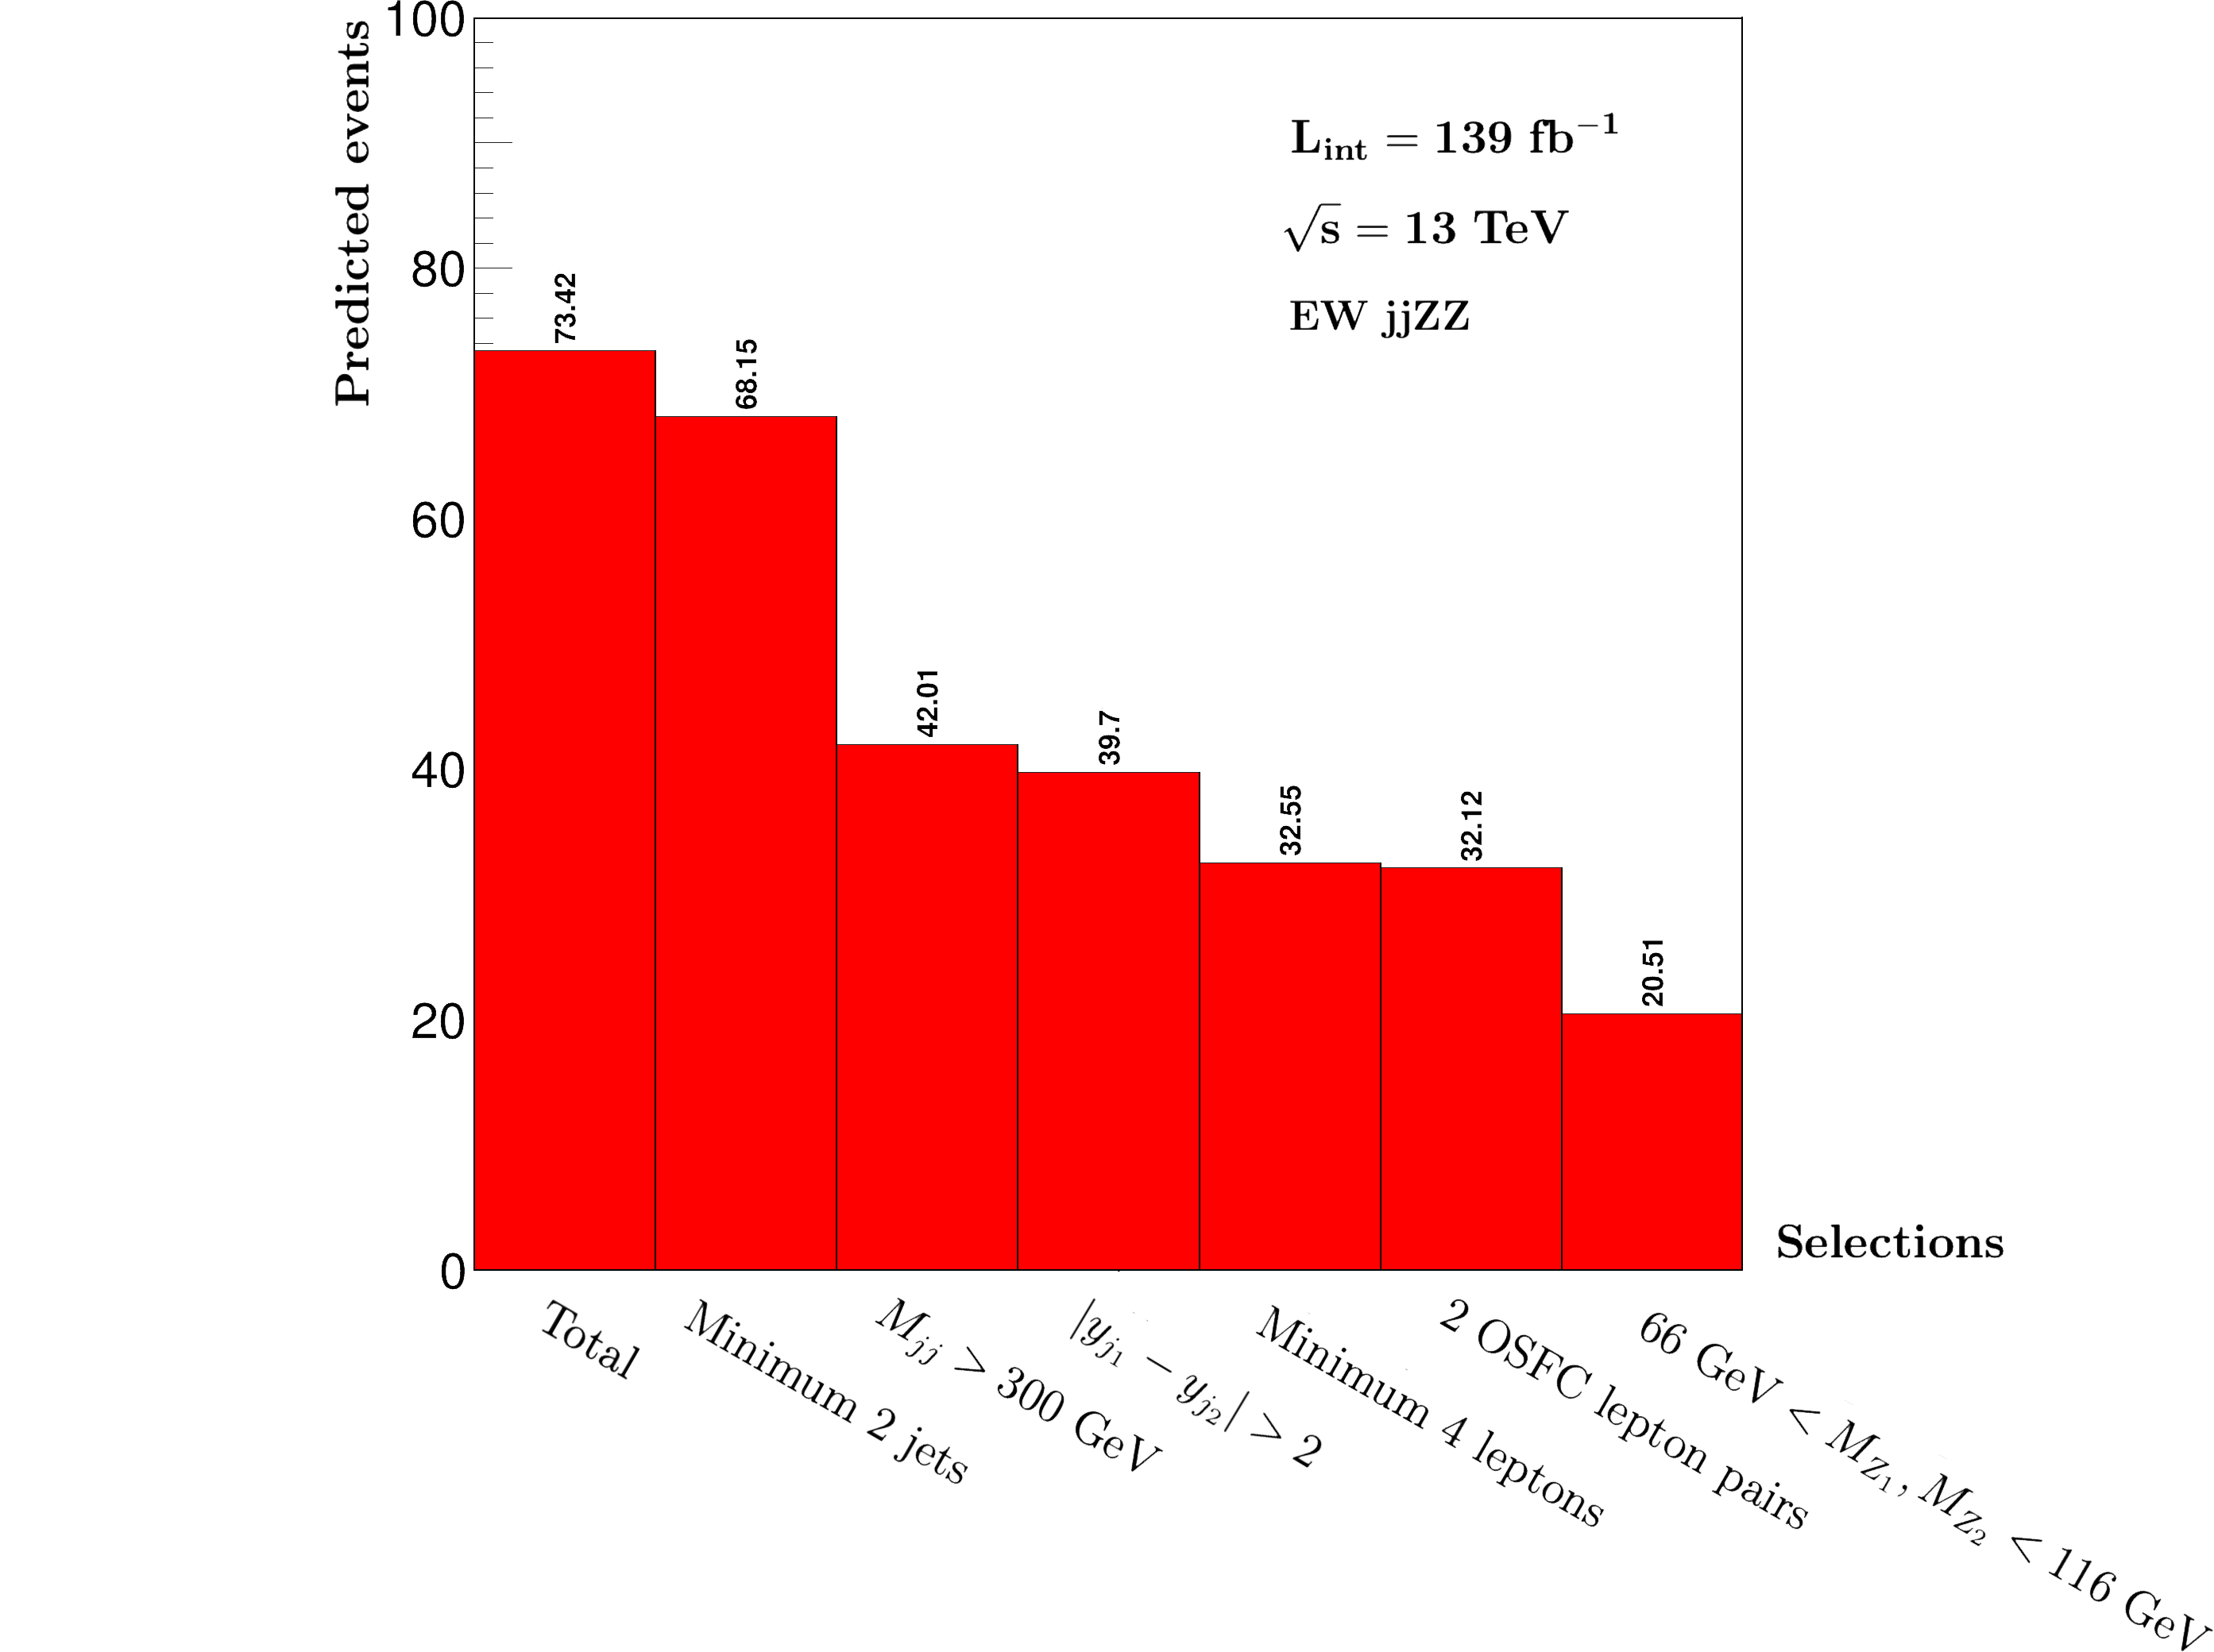
\includegraphics[scale=0.14]{ps/cutflow_stack.png}
            \caption{Cut-flow diagram of the predicted $EW\ jjZZ$ event number after selection cuts. Uncertainty was omitted and numbers after the decimal point were preserved.}
            \label{fig:cutflow}
            \end{centering}
        \end{figure}
        
    \section{Cut-flow comparison}
        \par In this measurement, three analysts worked on similar fiducial volumes, while developing different algorithm for events selection. 
        It is valuable to check the consistency of different implementations. A specific fiducial area and a particular order of selecting 
        physical objects were agreed and cut-flow diagrams indicating predicted $EW\ jjZZ$ event number based on simulation after 
        each selection are obtained. Only in this section, all three generations of simulation data were used, and the phase space volume 
        is slightly different from which is used in the measurement. Figure \ref{fig:cutflow} shows a cut-flow diagram which has been 
        compared with the other two analysts, and the result turns out to be consistent.
        
    \section{Background and uncertainty}
        \par The signal of $jjZZ4l$ channel contains three major processes, namely $EW\ ZZ4l$, $Strong\ qqZZ4l$ and $Strong\ ggZZ4l$; 
        In this stage of measurement, all processes were modelled using the simulation events. 
        The $VH$, tri-boson, $WZ$ process and processes with top quark in leading order can produce same or similar final state particles. 
        If leptons or jets were misidentified, they can potentially fake $jjZZ4l$ events, the dominate irreducible background is process 
        involving top quark, other contributions are small, all background processes are denoted ``Other'' process from now on. 
        In future analysis, data-driven methods can be used to estimate the background instead of using pure simulations.
        \begin{table}[ht!]
            \centering
            \renewcommand\arraystretch{1.2}
            \begin{tabularx}{\textwidth}{p{0.1405\textwidth} p{0.1405\textwidth}  p{0.1405\textwidth}  p{0.1405\textwidth}  p{0.1405\textwidth}  p{0.1405\textwidth} } 
            \hline\hline
            Process & Fiducial & SR & $\text{CR}_{C_{ZZ}}$ & $\text{CR}_{jIB}$ & $\text{CR}_{all}$\\
            \hline
            $EW\ ZZjj$ & $6.9\pm 0.04$ & $4.6\pm 0.03$ & $1.5\pm 0.02$ & $0.58\pm 0.01$ & $0.26\pm 0.01$ \\
            $QCD\ ggZZ$ & $7.00\pm 0.08$ & $3.7\pm 0.06$ & $1.4\pm 0.04$ & $1.3\pm 0.03$ & $0.49\pm 0.02$ \\
            $QCD\ qqZZ$ & $21.82\pm 0.22$ & $9.34\pm 0.16$ & $4.56\pm 0.08$ & $5.25\pm 0.12$ & $2.66\pm 0.06$\\
            $Other$ & $3.45\pm 0.17$ & $1.32\pm 0.11$ & $1.28\pm 0.09$ & $0.46\pm 0.08$ & $0.39\pm 0.03$\\
            \hline
            $Total$ & $39.17\pm 0.29$ & $18.99\pm 0.21$ & $8.77\pm 0.13$ & $7.60\pm 0.15$ & $3.81\pm 0.07$\\
            \hline
            $ Data$ & $42 \pm 6$ & $20\pm 4$ & $10\pm 3$ & $10\pm 3$ & $2\pm 1$\\
            \hline\hline
            \end{tabularx}
            \caption{Predicted and observed event number in fidutial region, SR and 3 CR regions, where the $S$ is short for $Strong$. Observation is compatible with the SM prediction. }
            \label{regevtstable}
        \end{table}
        \par With only selections of requiring at least two jets and four leptons, the predicted distribution 
        of 4-lepton invariant mass ($M_{4l}$) distribution is shown in Figure \ref{fig:finebined}, in which 
        the single Z boson resonance peak at around 91 GeV is dominated by $Strong\ qq4l$ processes, higgs resonance peak at around 125 GeV is dominated by 
        $Strong\ ggH4l$ processes, and the ``shoulder'' of Z bosons pair starting from about 182 GeV can be seen. In contrast, other background contributions 
        (yellow) is a small and relatively flat. The p-value of non-VBS hypothesis is defined as the probability of observed event number larger than $N_{data}$
        if the expected number of events do not include VBS events $p = P(N_{obs} > N_{data}\ |\ \mu_b)$. Since observed number satisfies Poisson distribution, 
        $p = 0.04$ the corresponding significance is calculated as $(N_{data} - \mu_b) = 1.5\sigma_{N_{data}}$
        \begin{figure}[ht]
            \begin{centering}
            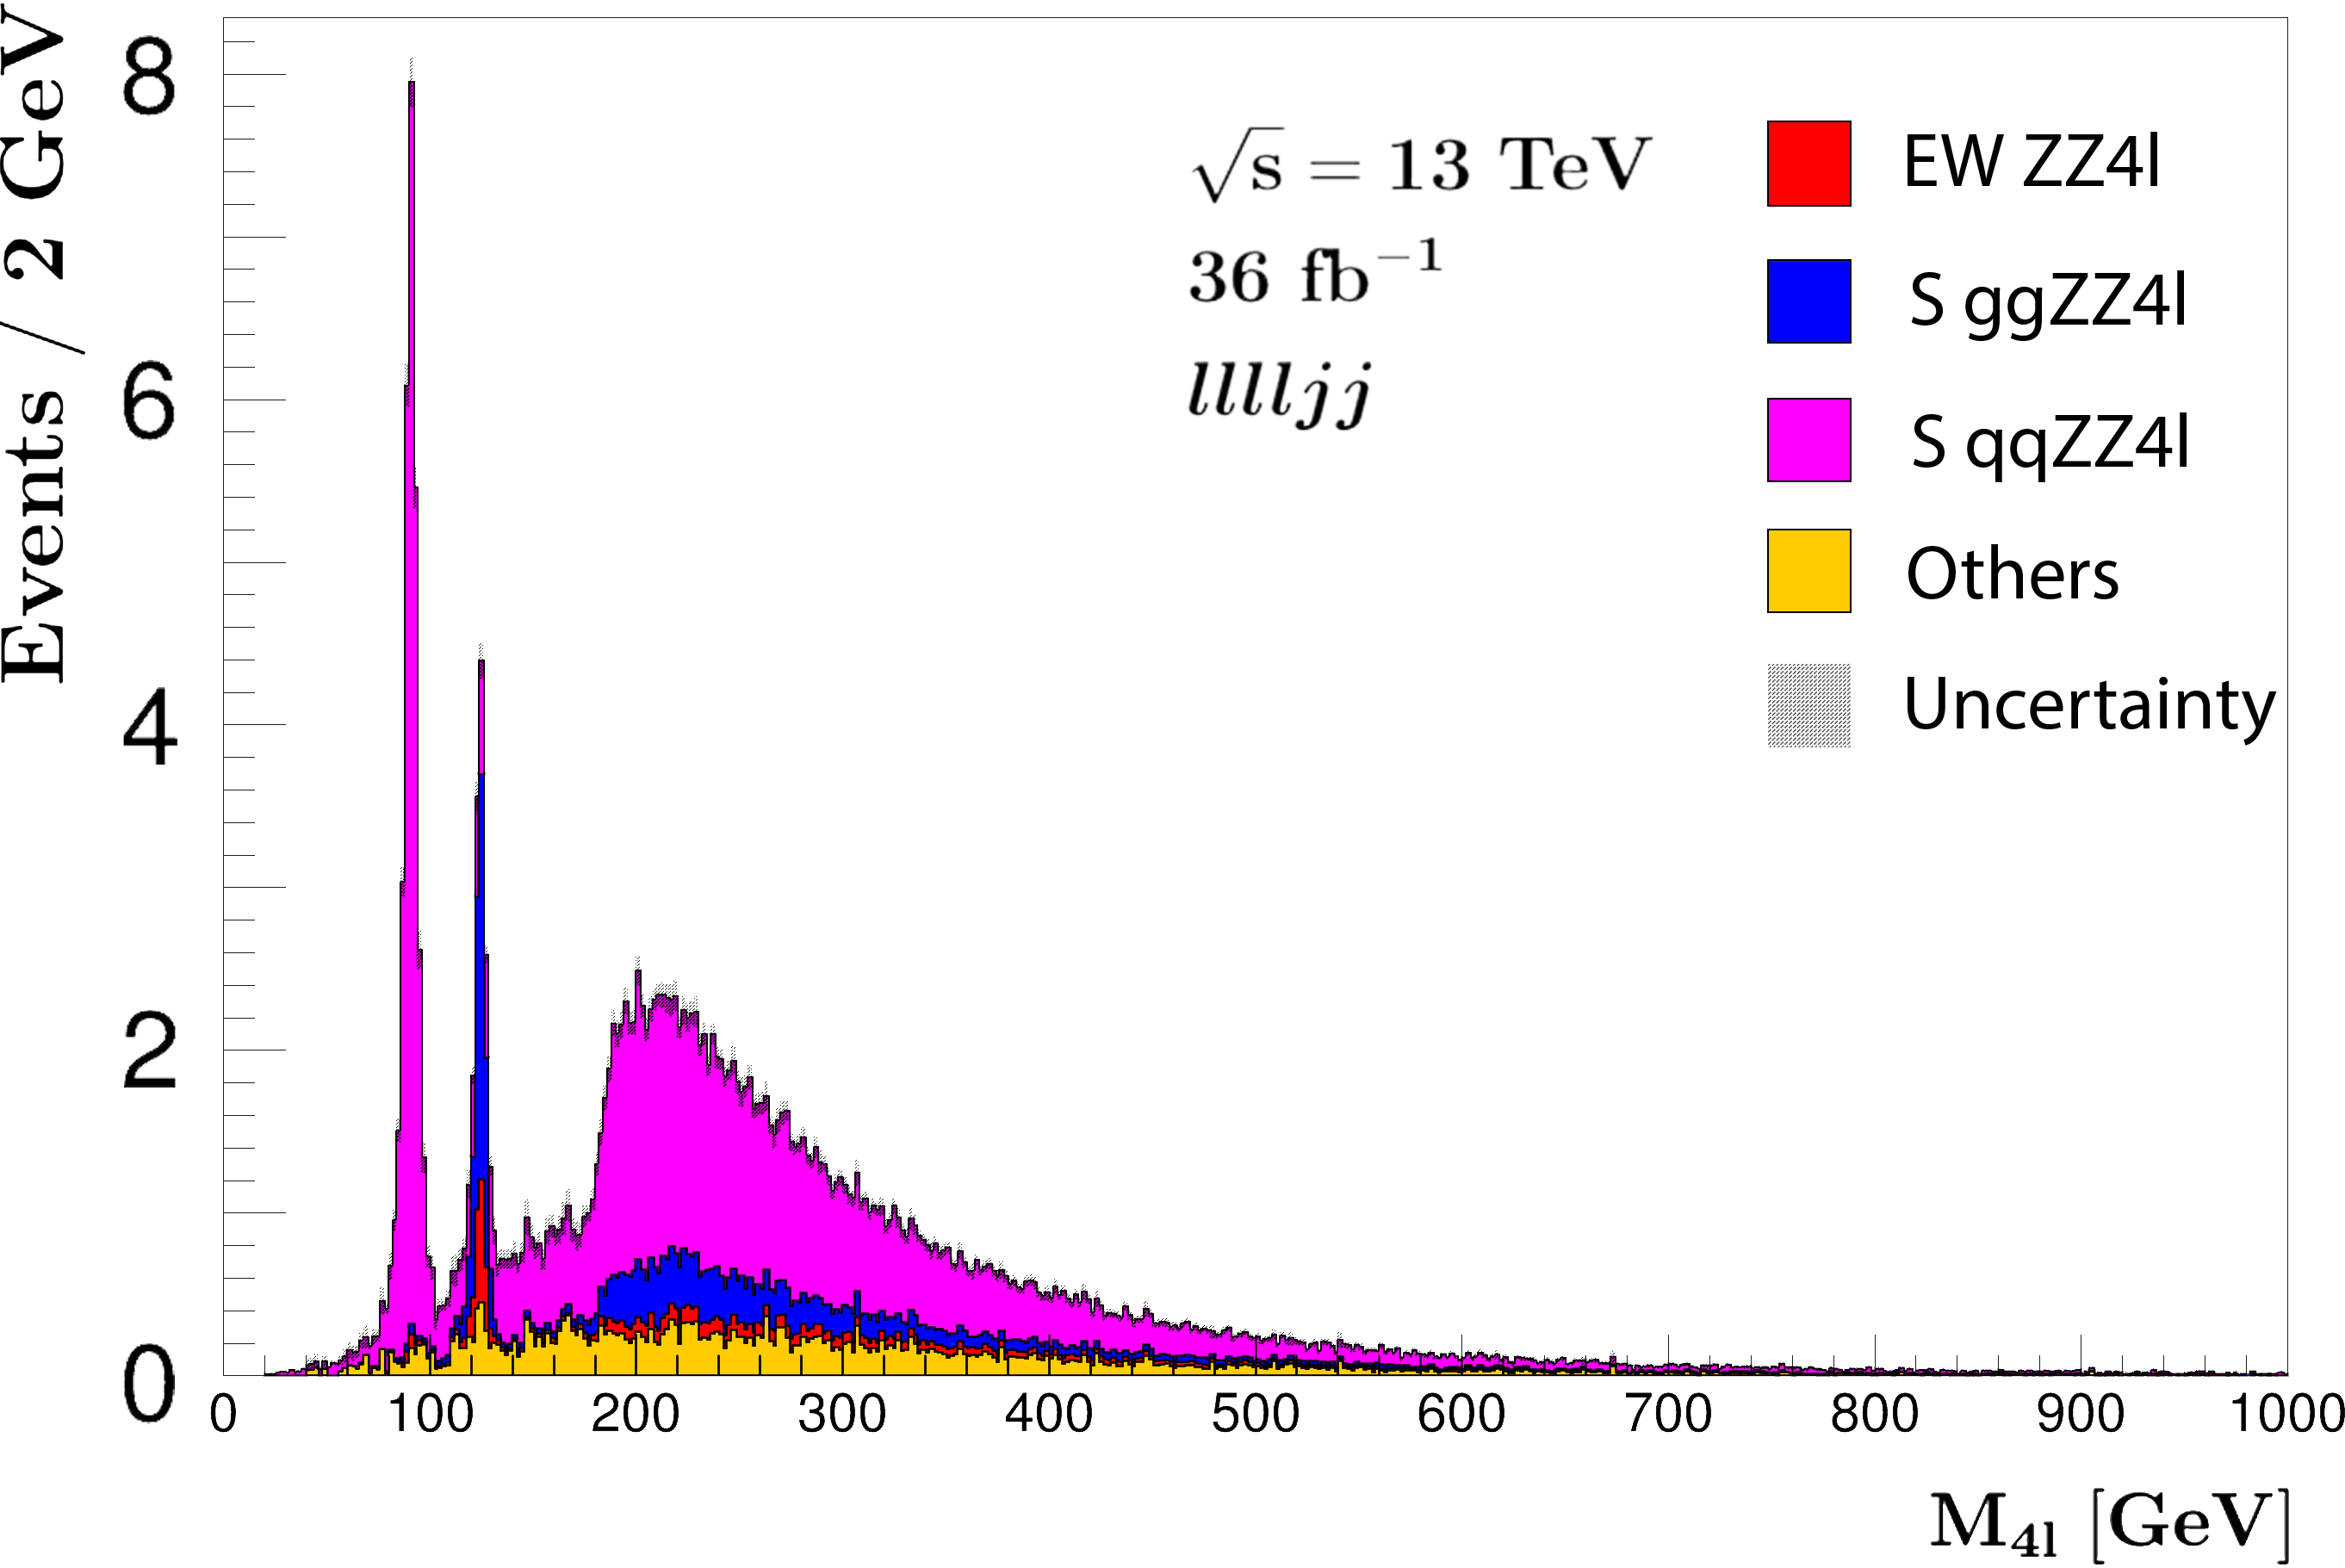
\includegraphics[scale=0.12]{ps/det_llll_m_stack.png}
            \caption{Predicted detector-level $M_{4l}$ distribution with very fine binning, main resonance features are shown clearly.}
            \label{fig:finebined}
            \end{centering}
            
        \end{figure}
        \par The number of expected and observed detector-level events in different regions defined are listed in 
        table \ref{regevtstable}, where the consistency between the data and the SM prediction is shown. 
        The uncertainties shown in the table only includes statistical errors, further work is needed to 
        identify sources of systematical uncertainties, which contain the modelling error of simulation data, 
        the interference between processes and the uncertainties due to the experimental limits. 
        Due to low events yield, the inclusive fiducial region was used to perform rest measurements, 
        the predicted $M_{4l}$ and $M_{jj}$ distributions overlayed with the observed data in the fiducial region are shown in Figure \ref{fig:simpleconsist}        
        \begin{figure}[ht]
            \begin{centering}
            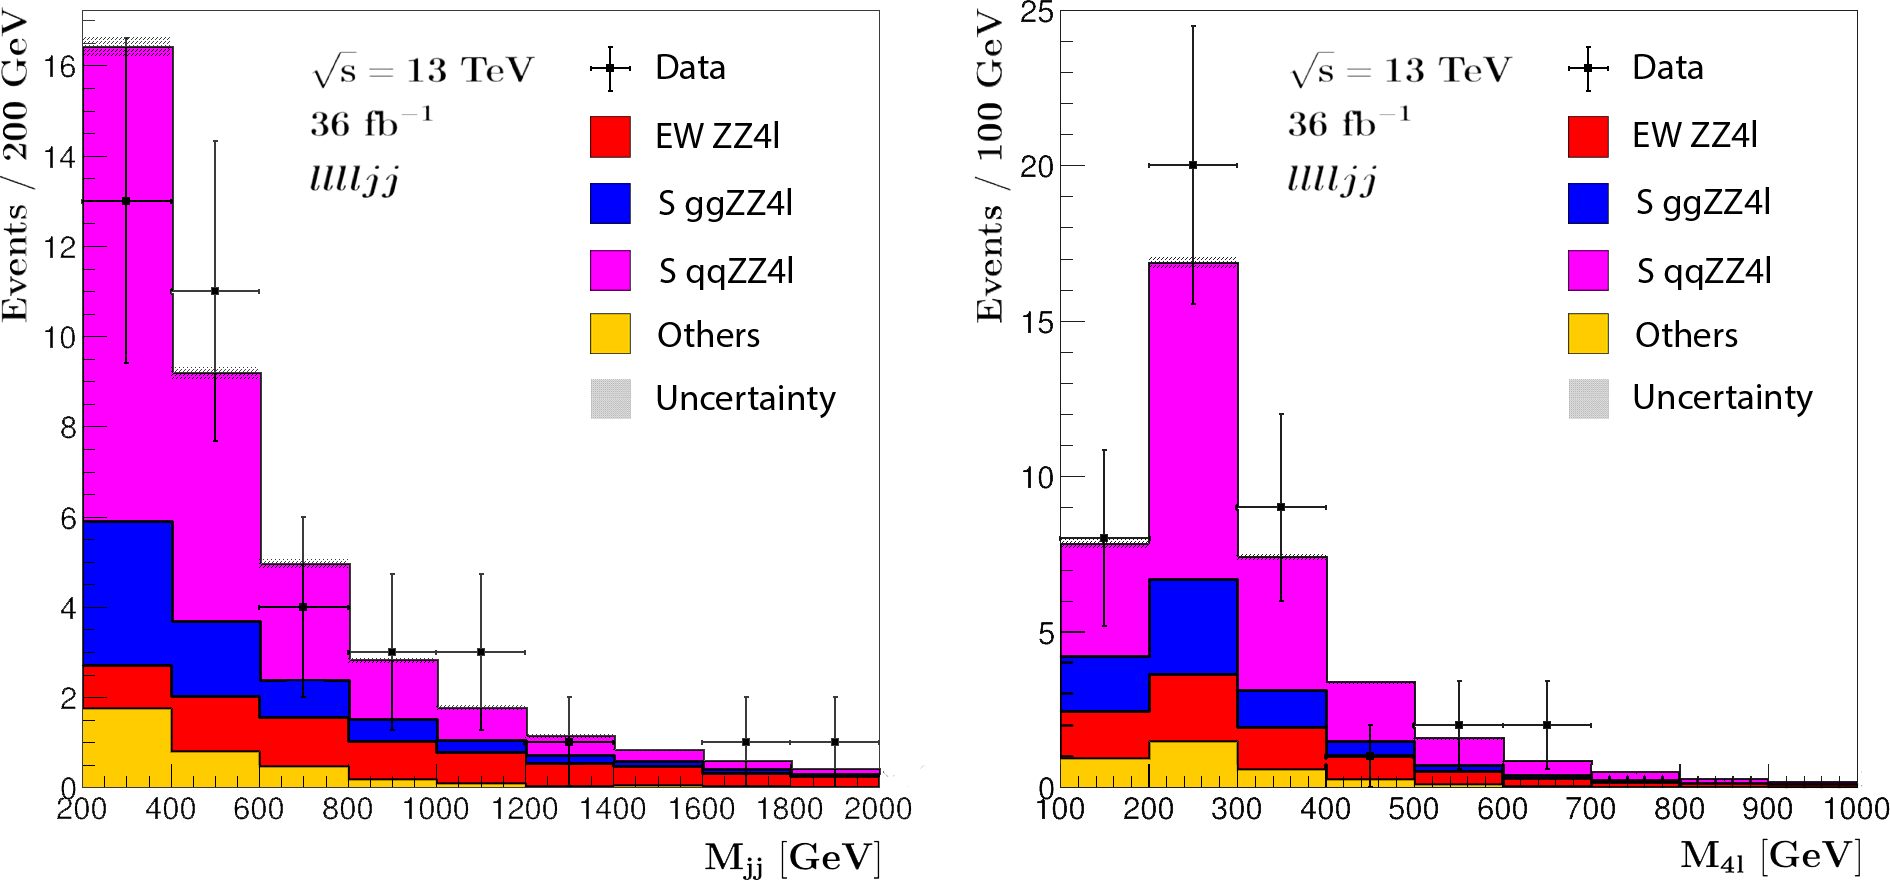
\includegraphics[scale=0.225]{ps/mjj_m4l_equalbins.png}
            \caption{the predicted and observed $M_{4l}$, $M_{jj}$ distribution, showing that the observation is consistent with the SM prediction.}
            \label{fig:simpleconsist}
            \end{centering}
        \end{figure}
    
    \section{Unfolding}
        \par The measured spectrums were ``unfolded'' to correct for detector effects\cite{refId0}, for example, the inefficiency, 
        limited resolution and events migration caused by the detector and triggers. The unfolding technique allows 
        the measurement to be directly compared with theory predictions without knowing experimental details
        so that the BSM benchmark models can be easily injected into the result. Moreover, future experiments 
        in the same fiducial region can also be compared directly for consistency check. These features make a measurement
        with detector effect removed a ``model-independent'' measurement.       
        \subsection{Theory framework}
            \par The unfolding technique relies on information of how the particle-level (truth-level) events were measured and 
            formed the detector-level (measurement-level) distributions, in other words, how the detector alter the true distribution. 
            The detector effect is described by three key components:\newline
            \textbf{The reconstruction efficiency $\mathbf{\epsilon{^{i}}}$} is defined as the probability of truth-level events in bin i pass the truth-level 
            selection but failed to pass detector-level selection.
            $$\epsilon^{i} = P(\text{event not measured}\ |\ \text{true value in bin i})$$
            the inefficiency is caused by the inefficiency of the trigger and the detector, as well as events that migrate out of the 
            region in the detector-level.\newline
            \textbf{The migration matrix $R^{ij}$} is measured as the fraction of truth-level events in bin i founded in bin j in the detector-level.
            $$R^{ij} = P(\text{event measured in bin j}\ |\ \text{true value in bin i})$$
            The non-diagonal part ($i\neq j$) indicates the probability of events migration, while the diagonal part $R^{ii}$ in the response matrix is also called the purity, 
            which indicates the ratio of events that do not migrate. The cause of migration is the limited resolution and accuracy of the detector.\newline
            \textbf{The fake ratio $F^i$} is defined as the ratio of events that pass detector-level selection but cut off in the truth-level over the number of events in truth-level bin i.
            $$F^j = P( \text{event measured in bin j}\ |\ \text{no truth-level correspondent})$$
            A faked event can occur if the detector miss identifies particles from another event.
            \par If the migration can be ignored, $R^{ij} \sim I$, one can simply perform a bin-by-bin method to unfold, using
            $$N_{meas}^i -  N_{meas}^i F^{i} = N_{true}^i {\epsilon^{i}}$$
            rearrange the equation gives
            $$N_{true}^i = \frac{N_{meas}^i(1-F^i)}{{\epsilon^{i}}}$$
            If migration cannot be ignored, it is possible to add a migration removal process by inverting $R^{ij}$
            $$N_{meas}^i  - N_{meas}^i F^{i} = {\epsilon^{i}}\sum_{j}^{all\ bins}R^{ij} N_{true}^j$$
            It is clear that in order to get $N_{true}^i$, inversion of the response matrix is required.
            consider a perfect distribution with no fake and no inefficiency, the equation above gives
            $$(R^{-1})^{ij}N^i_{meas} = N^j_{true}$$
            where summation convention over j is used, and $N^{i}$, $(R^{-1})^{ij}$ represents vector and matrix.
            Unfortunately, this is a rather strong condition as $det(R^{ij})\neq0$ is not guaranteed for a measured distribution.
            Even if $R^{ij}$ can be inverted, this method is not able to handle large statistical fluctuation as the inversion 
            of a matrix can contain negative values. 
            \par Consider an arbitrary observable distribution which obey normal distribution with 
            $\sigma=1$ and $x_0 = 0$, due to limited resolution,  detector-level events was altered by a random gaussian function with 
            $\sigma=0.2$ and $x_0 = 0$. Given no detector inefficiency nor faked event but with fairly high statistical fluctuation, 50 events were generated. 
            Figure \ref{fig:demounfreverse} shows the result of the matrix inversion method on this example distribution.
            \begin{figure}[ht]
                \begin{centering}
                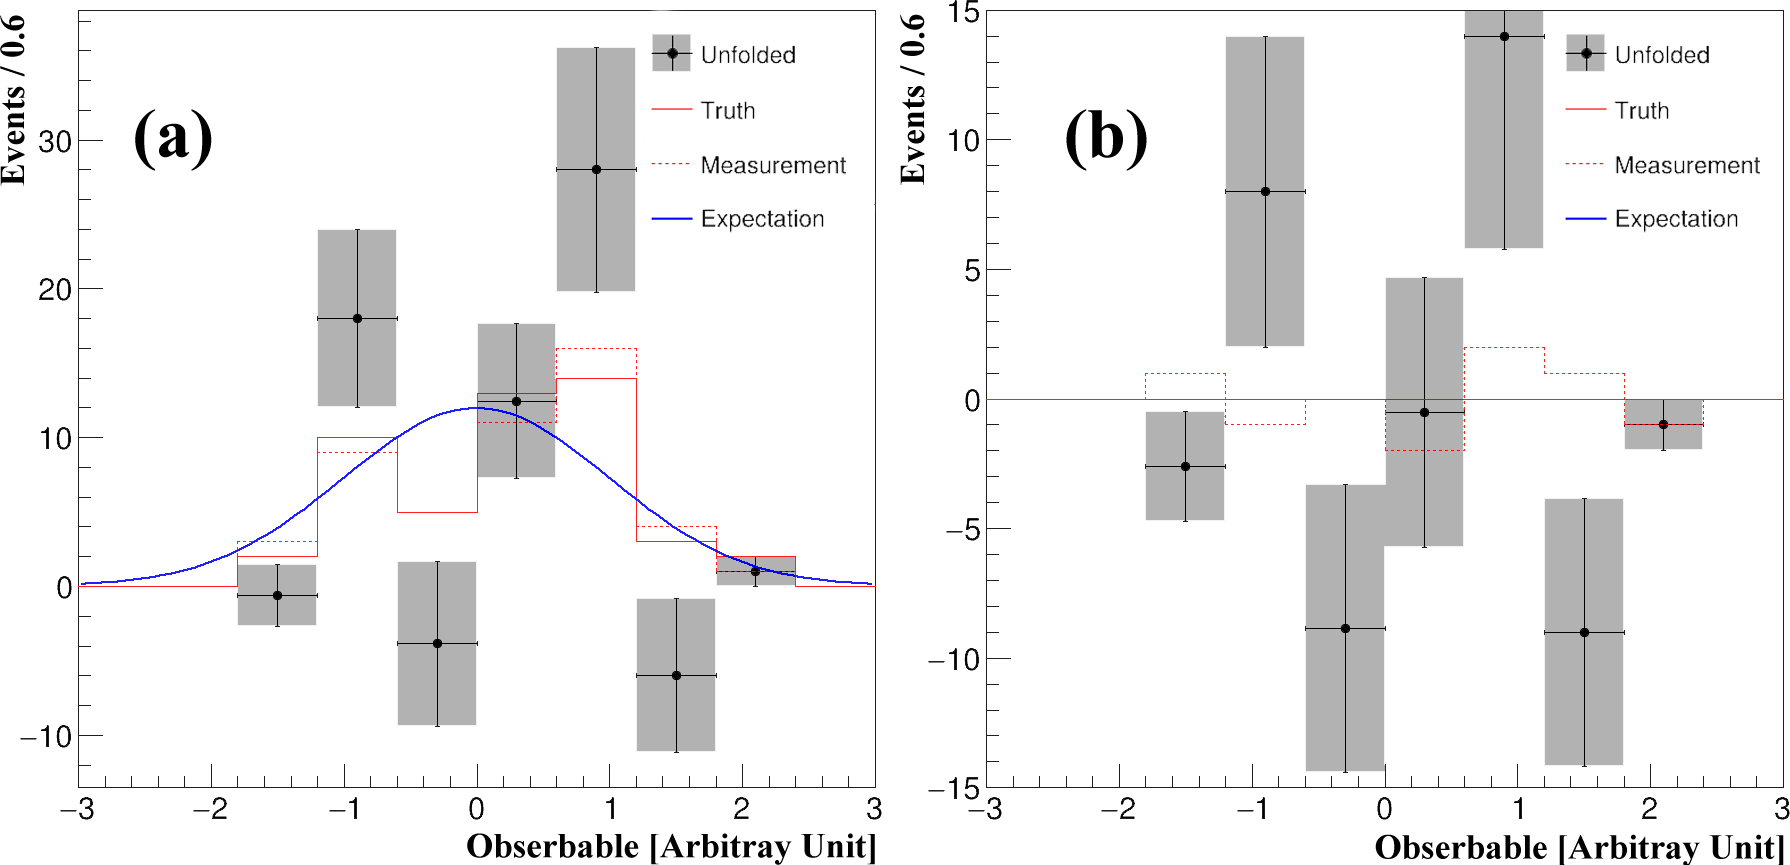
\includegraphics[scale=0.23]{ps/unfold_demo.png}
                \caption{Unfolding result of an example distribution with high statistical fluctuation using the matrix inversion method.
                \textbf{(a)} the inversion method shows a large deviation from the truth due to unstable inverted response matrix. \textbf{(b)} the difference between the unfolded spectrum and true distribution.}
                \label{fig:demounfreverse}
                \end{centering}
            \end{figure}
            \par An iterative unfolding method based on Baye's theorm\cite{DAgostini:1994fjx}\cite{DAgostini2010ImprovedIB} can solve this problem, 
            the best estimation of $N^i_{true}$ is updated iteratively by 
            $$\hat{N}^i_{true} = \frac{1}{\epsilon^i}\sum_{j}(\frac{R^{ij}p^i}{\sum_{k}R^{jk}p^k})N^j_{meas}(1-F^j)$$
            where the first iteration $p_i$ is given by $\hat{N}^i_{true}=N_{total}p^i$. The updated estimation of 
            $N^i_{true}$ can be compared with the previous estimation; if the change is large, another iteration can be performed 
            based on the current estimator. However, continuing to iterate brings increasingly large variation and the 
            estimators approach to the unstable solution from matrix inversion\cite{Cowan:2002in}. However, the smaller the iteration, 
            The more biased the result is. This method is applied to the same distribution as stated previous, 
            much better performance is achieved and shown in figure \ref{fig:demounfbayes}.
            \begin{figure}[ht]
                \begin{centering}
                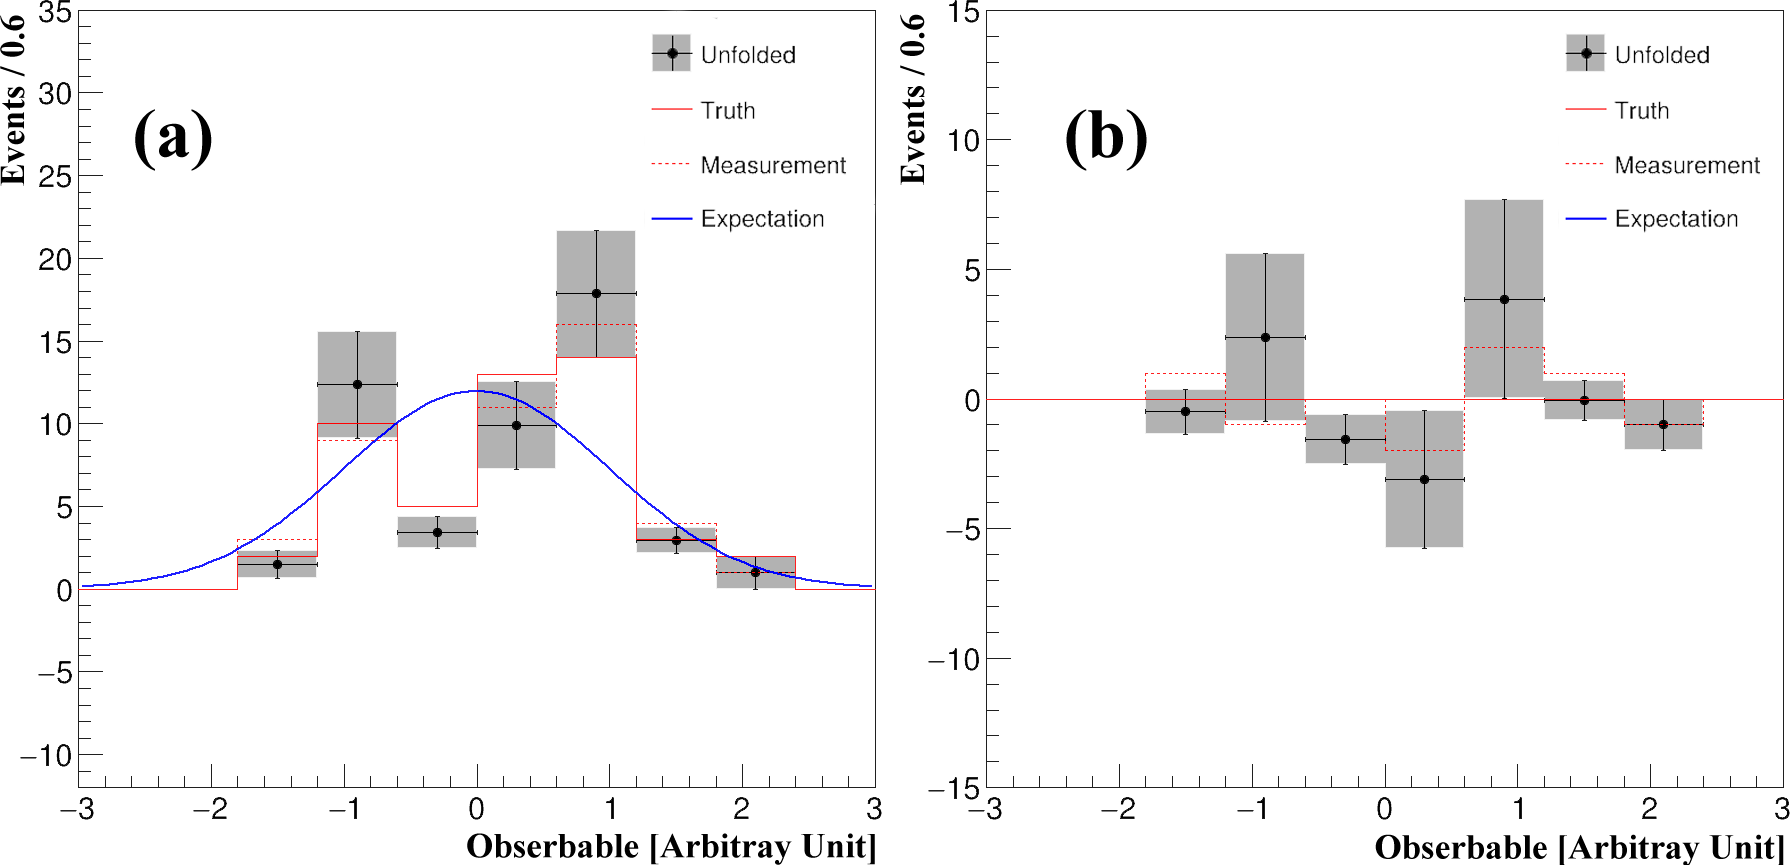
\includegraphics[scale=0.23]{ps/unfold_demo_bayes.png}
                \caption{Unfolding result on the same example distribution as previous using the iterative method with one iteration, 
                higher iteration will result in a similar issue as seen in figure \ref{fig:demounfreverse}.
                \textbf{(a)}The performance of unfolding is much better than the inversion method. 
                \textbf{(b)} The oscillation of the estimation is largely suppressed by the iterative method.}
                \label{fig:demounfbayes}
                \end{centering}
            \end{figure}
        \subsection{Distributions and results}
            \par In this measurement, three distributions of observables were measured and unfolded, $M_{jj}$, $M_{4l}$ and $\Delta{\phi}_{jj}$.
            While the first two are defined as above, $\Delta{\phi}_{jj}$ is a CP sensitive observable defined as 
            $$\Delta{\phi}_{jj} = \phi_{j_1} - \phi_{j_2}$$ 
            where $\phi_{J_{1,2}}$ is the azimuthal angle of the two jets selected, the order (1,2) is arranged according to the rapidities of 
            the two jets, so that $j_i$ is always the most forwarding jet in space. The asymmetry in positive and negative region of $\Delta{\phi}_{jj}$ 
            distribution is a probe of CP violation\cite{Bernlochner_2019}, which is defined as 
            $$A = \frac{N(0<\Delta{\phi}_{jj} <\pi) - N(-\pi<\Delta{\phi}_{jj} <0)}{N(0<\Delta{\phi}_{jj}<\pi) + N(-\pi<\Delta{\phi}_{jj} <0)}$$

            \par Due to limited event yields in the fiducial region, the binning of the distribution is determined using the simulation 
            data by requiring at least 10 events of inclusive $jjZZ4l$ events per bin in detector-level simulation, the higgs region 
            bin in $M_{4l}$ distribution ($110\ \text{GeV} < M_{4l}< 140\ \text{GeV}$) is hard-coded to show the higgs contribution, 
            and the bin of $\Delta{\phi}_{jj}$ is manually set to be symmetric over 0. The prediction of background processes is then 
            used to subtract the none $jjZZ$ process in the observed data. The response matrix, efficiency and fake rate is calculated 
            by simulation in truth and detector-level using RooUnfold package\cite{adye2011unfolding}. Finally, the iterative unfolding 
            method is performed on each distribution based on this information. One iteration is found to be optimal for all distributions 
            due to high purities in all three distributions. The response matrices and unfolding results of the three distributions are 
            shown in figure \ref{fig:delredi} \ref{fig:mjjredi} \ref{fig:m4lredi}.            
            \begin{figure}[ht]
                \begin{centering}
                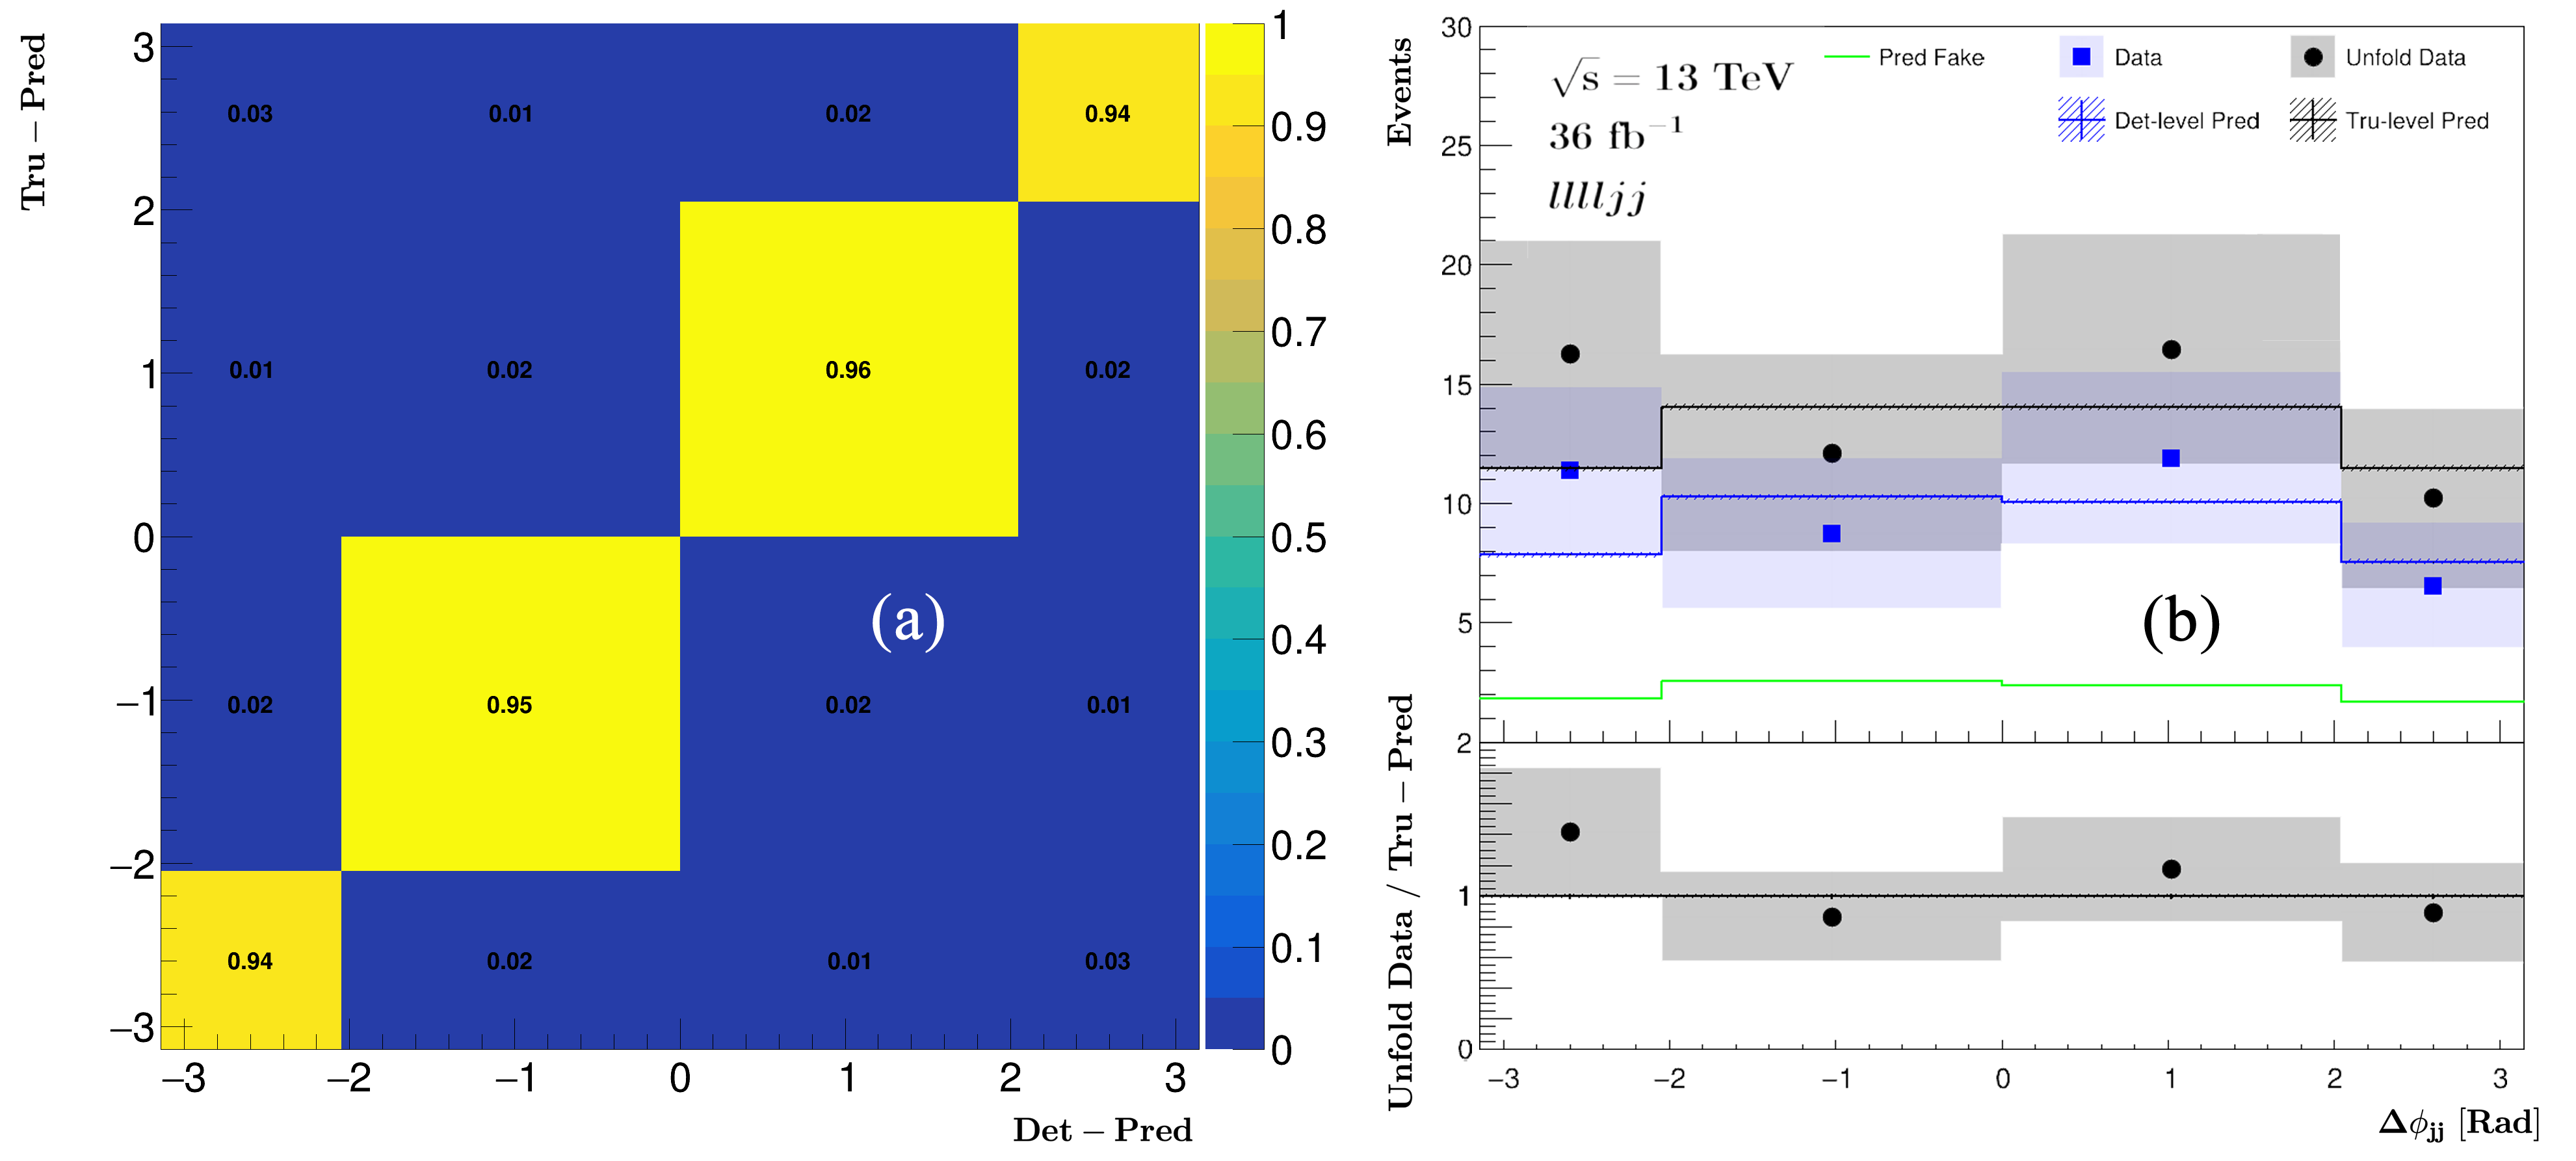
\includegraphics[scale=0.108]{ps/del_redi.png}
                \caption{\textbf{(a)} Predicted response matrix for $\Delta\phi_{jj}$ distribution in the fiducial region, where Det-Pred and Tru-Pred are detector-level and truth-level prediction respectively.
                High purity is shown in this region. \textbf{(b)} The detector-level data and prediction, truth-level prediction and the result of the iterative unfolding method with one iteration on $\Delta\phi_{jj}$ distribution, both detector and truth level result are showing consistency with SM prediction.}
                \label{fig:delredi}
                \end{centering}
            \end{figure}
            \begin{figure}[ht]
                \begin{centering}
                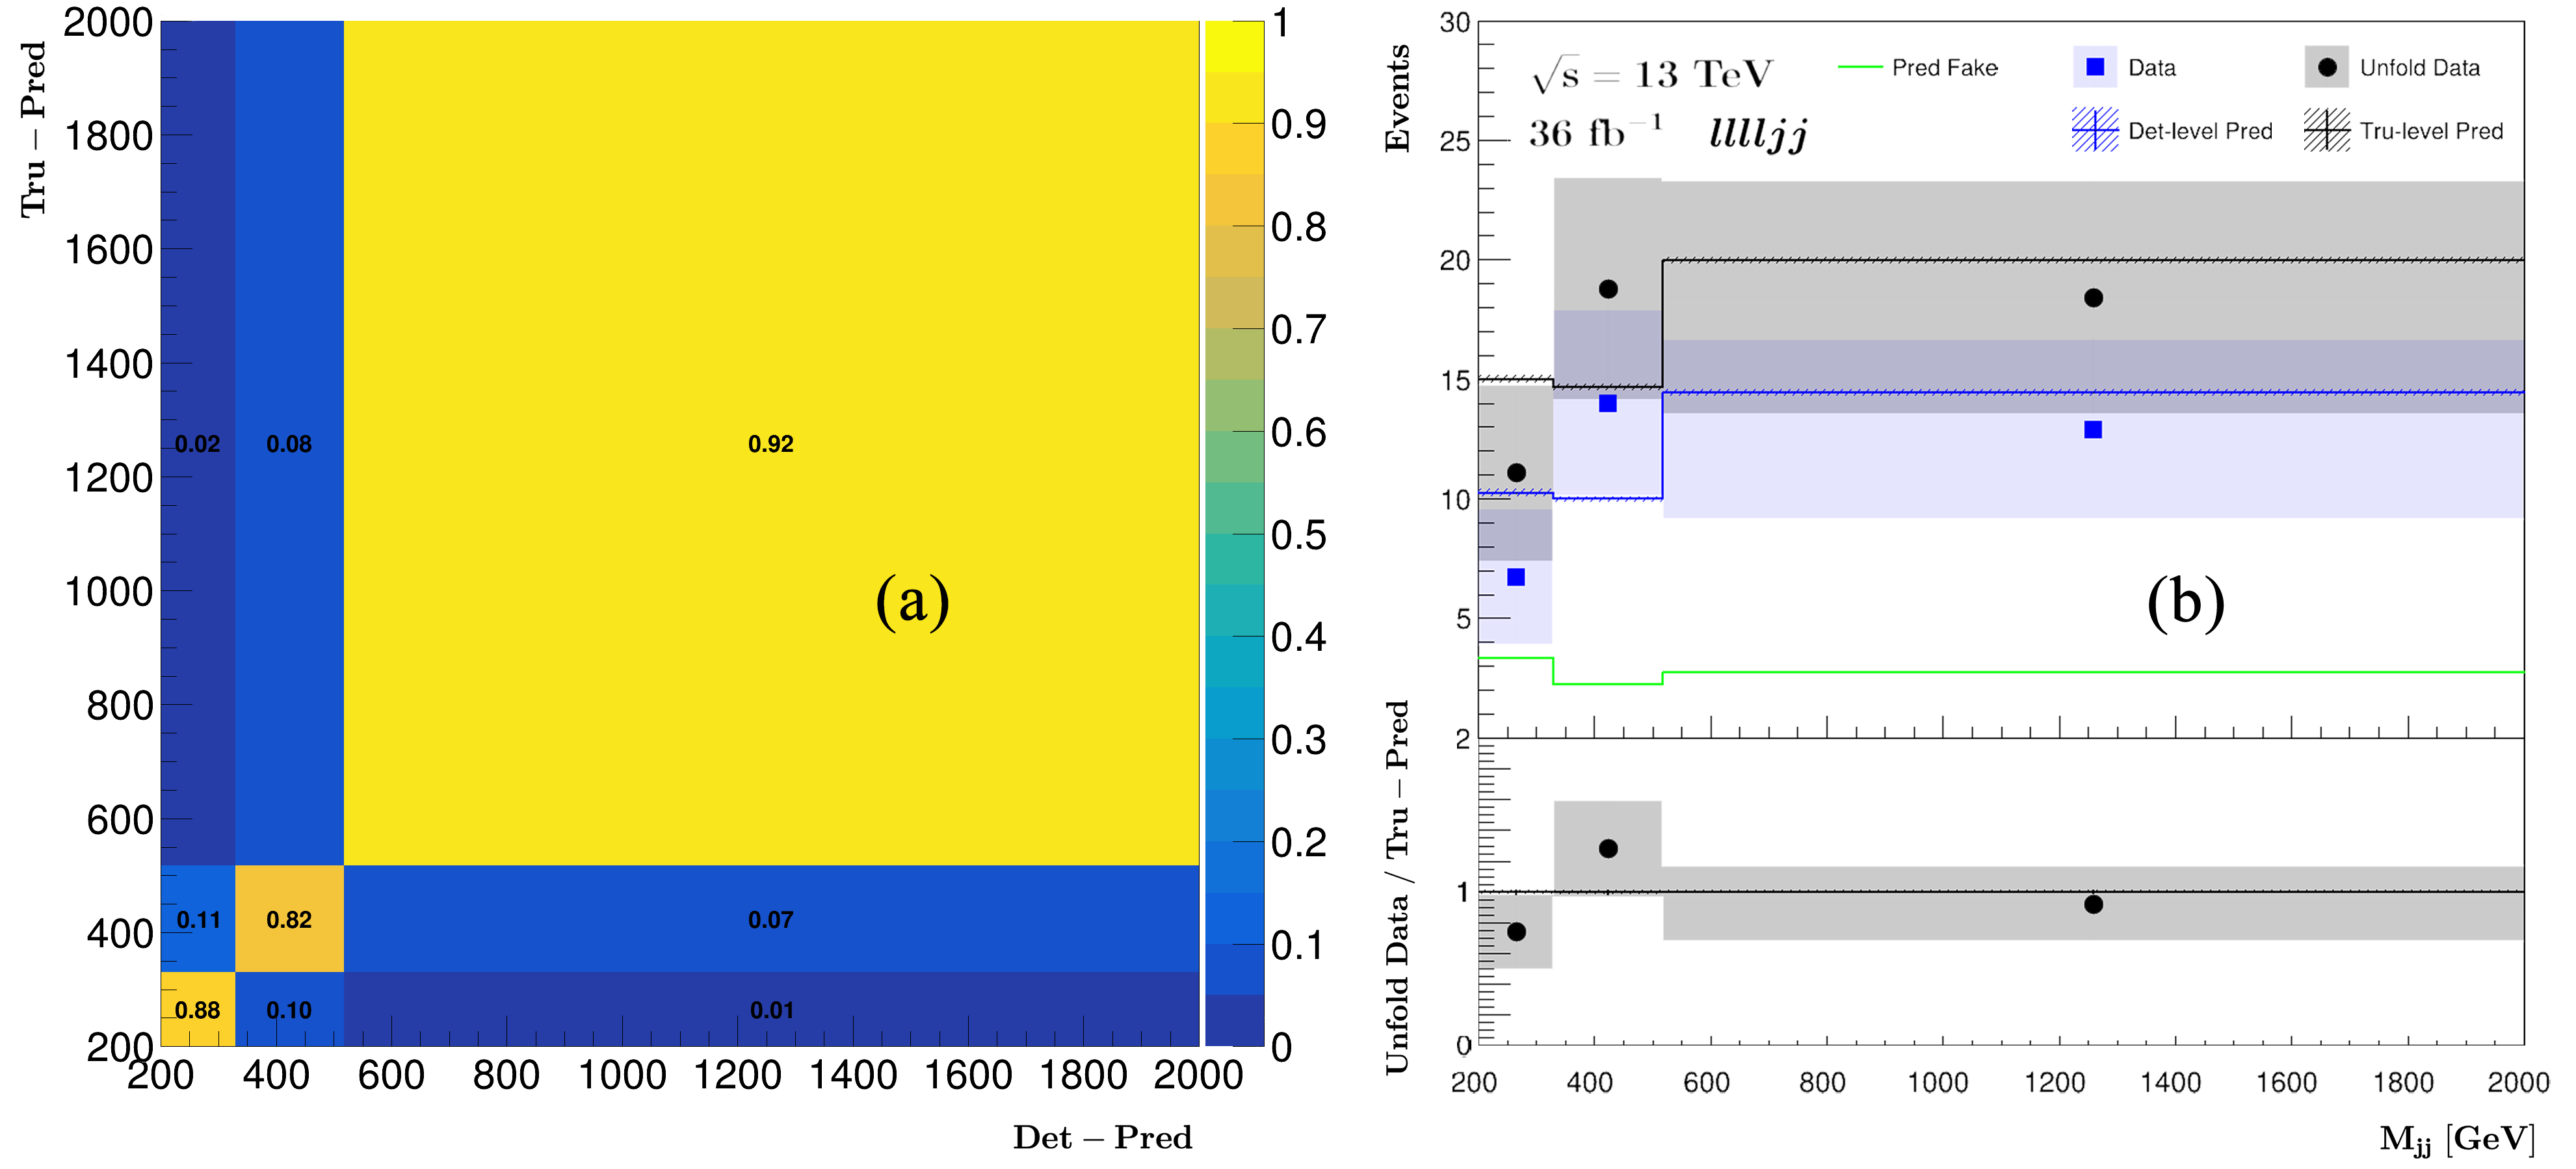
\includegraphics[scale=0.108]{ps/mjj_redi.png}
                \caption{\textbf{(a)} Predicted response matrix for $M_{jj}$ distribution in the fiducial region, high purity is shown too. 
                \textbf{(b)} The detector-level data and prediction, truth-level prediction and the result of unfolding with the same method used in the $\Delta\phi_{jj}$ spectrum, both detector and truth level result are showing consistency with SM prediction.}
                \label{fig:mjjredi}
                \end{centering}
            \end{figure}
            \begin{figure}[ht]
                \begin{centering}
                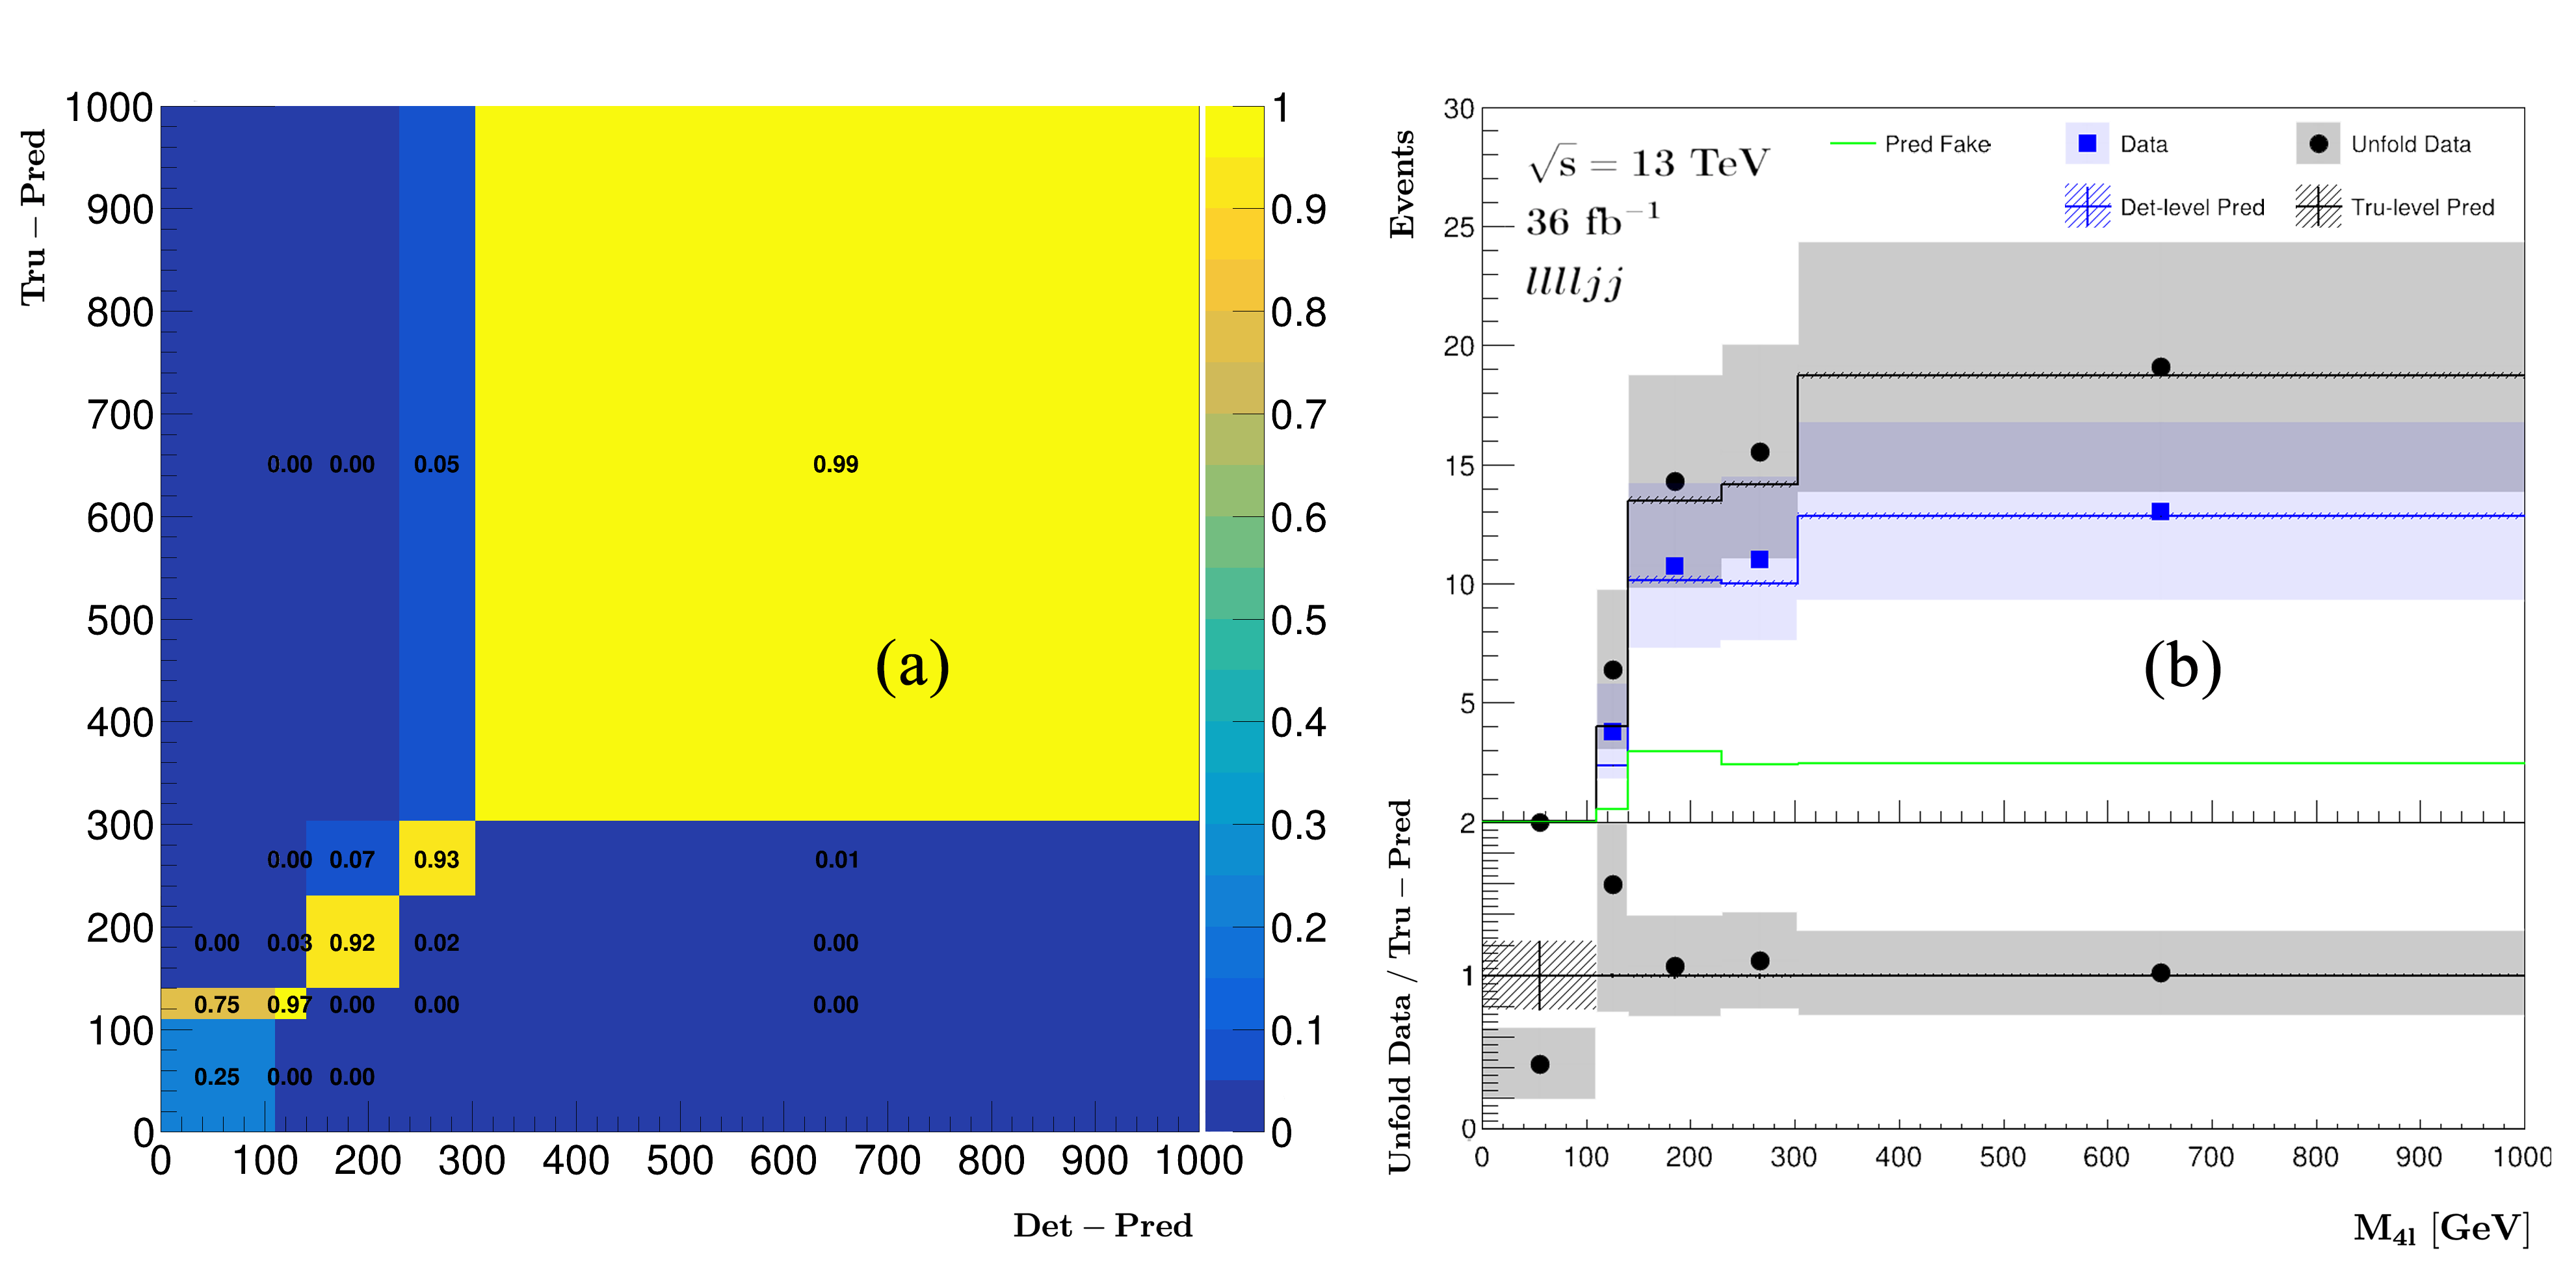
\includegraphics[scale=0.108]{ps/m4l_redi.png}
                \caption{\textbf{(a)} Predicted response matrix for $M_{jj}$ distribution in the fiducial region, the only one bin gives low purity come from the detector migration from higgs region.
                \textbf{(b)} The detector-level data and prediction, truth-level prediction and the result of unfolding using the same method used in the $\Delta\phi_{jj}$ spectrum, both detector and truth level result are showing consistency with SM prediction.}
                \label{fig:m4lredi}
                \end{centering}
            \end{figure}
            \par As can be seen in the response matrices, all distributions have a very high purity level since the bin 
            width is much larger than the resolution of the detector. The only one bin that has low purity is the first 
            bin of the $M_{4l}$ spectrum, which is caused by the Z-mass selections (see Table \ref{selectioncut}) in 
            the fiducial region excluded events with 4-lepton invariant mass lower than Z mass, these events shown in 
            the first bin in detector-level are migrated from the higgs region in the truth-level.
    \section{Result}
        \par With the infrastructure in hand, the geometrical asymmetry $A$ and the inclusive $jjZZ4l$ cross-section in the 
        fiducial region defined as $\sigma^{fid}_{jjZZ4l} = N^{unfold}_{jjZZ4l}/ L_{int}$ can be measured, where the $N^{unfold}_{jjZZ4l}$ 
        is the unfolded result in the fiducial region, $L_{int}$ is the integrated luminosity $36fb^{-1}$ corresponding to 
        the data. The asymmetry is measured to be $A = -0.03 \pm 0.16$, which is consistent with the prediction $A_{pred} = -0.000 \pm 0.005$. 
        The fiducial cross-section is found to be $\sigma^{fid}_{jjZZ4l} = 1.53 \pm 0.24$, which is also compatible with the 
        SM prediction $\sigma^{fid}_{jjZZ4l} = 1.416 \pm 0.007$. The significance of $EW\ jjZZ$ production is $1.5$ with corresponding p-value $0.04$.
        The uncertainties here are statistical only.

    \section{Conclusion}
        \par The result of the measurement shows good consistency with the SM prediction, showing the great success of 
        the SM theory and MC simulations technique. However, with the data corresponding to an integrated luminosity 
        of $3000fb^{-1}$ expected to be delivered by the HL-LHC\cite{ATL-PHYS-PUB-2019-005}, the statistical uncertainty 
        is expected to be 10 times lower compared to the $36fb^{-1}$ data, opening the chance of scrutiny of the SM with 
        much higher accuracy. Moreover, the SR and CR are predicted to have the ability to separate the EW and Strong 
        events of jjZZ production, more statistics will enable us to check the pure EW VBS process separately. 
        With only little data, the unfolding method enables us to set limits of various benchmark theories beyond the 
        SM using the confidence level ($CL_s$) technique\cite{Read_2002}. 
        \par In the next term, the total of $139fb^{-1}$ of pp collision data collected in the ATLAS detector will be available; I am
        confident that evidence, even observation of $EW\ jjZZ$ process can be seen.
        The main objectives next year are estimating the systematical uncertainties and check and optimise the model sensitivity 
        to the BSM theories. 
        $$\mathbf{Events\ /\ \frac{\pi}{4}}$$
        $$\mathbf{\Delta\phi_{jj}\ [rad]}$$
    \bibliographystyle{unsrt}
    \bibliography{bibli.bib}
    
\end{document}